\documentclass[twoside]{book}

% Packages required by doxygen
\usepackage{fixltx2e}
\usepackage{calc}
\usepackage{doxygen}
\usepackage[export]{adjustbox} % also loads graphicx
\usepackage{graphicx}
\usepackage[utf8]{inputenc}
\usepackage{makeidx}
\usepackage{multicol}
\usepackage{multirow}
\PassOptionsToPackage{warn}{textcomp}
\usepackage{textcomp}
\usepackage[nointegrals]{wasysym}
\usepackage[table]{xcolor}

% NLS support packages
%\usepackage{hfont}
\usepackage{kotex}

% Font selection
\usepackage[T1]{fontenc}
\usepackage[scaled=.90]{helvet}
\usepackage{courier}
\usepackage{amssymb}
\usepackage{sectsty}
\renewcommand{\familydefault}{\sfdefault}
\allsectionsfont{%
  \fontseries{bc}\selectfont%
  \color{darkgray}%
}
\renewcommand{\DoxyLabelFont}{%
  \fontseries{bc}\selectfont%
  \color{darkgray}%
}
\newcommand{\+}{\discretionary{\mbox{\scriptsize$\hookleftarrow$}}{}{}}

% Page & text layout
\usepackage{geometry}
\geometry{%
  a4paper,%
  top=2.5cm,%
  bottom=2.5cm,%
  left=2.5cm,%
  right=2.5cm%
}
\tolerance=750
\hfuzz=15pt
\hbadness=750
\setlength{\emergencystretch}{15pt}
\setlength{\parindent}{0cm}
\setlength{\parskip}{3ex plus 2ex minus 2ex}
\makeatletter
\renewcommand{\paragraph}{%
  \@startsection{paragraph}{4}{0ex}{-1.0ex}{1.0ex}{%
    \normalfont\normalsize\bfseries\SS@parafont%
  }%
}
\renewcommand{\subparagraph}{%
  \@startsection{subparagraph}{5}{0ex}{-1.0ex}{1.0ex}{%
    \normalfont\normalsize\bfseries\SS@subparafont%
  }%
}
\makeatother

% Headers & footers
\usepackage{fancyhdr}
\pagestyle{fancyplain}
\fancyhead[LE]{\fancyplain{}{\bfseries\thepage}}
\fancyhead[CE]{\fancyplain{}{}}
\fancyhead[RE]{\fancyplain{}{\bfseries\leftmark}}
\fancyhead[LO]{\fancyplain{}{\bfseries\rightmark}}
\fancyhead[CO]{\fancyplain{}{}}
\fancyhead[RO]{\fancyplain{}{\bfseries\thepage}}
\fancyfoot[LE]{\fancyplain{}{}}
\fancyfoot[CE]{\fancyplain{}{}}
\fancyfoot[RE]{\fancyplain{}{\bfseries\scriptsize 다음에 의해 생성됨 \+:  Doxygen }}
\fancyfoot[LO]{\fancyplain{}{\bfseries\scriptsize 다음에 의해 생성됨 \+:  Doxygen }}
\fancyfoot[CO]{\fancyplain{}{}}
\fancyfoot[RO]{\fancyplain{}{}}
\renewcommand{\footrulewidth}{0.4pt}
\renewcommand{\chaptermark}[1]{%
  \markboth{#1}{}%
}
\renewcommand{\sectionmark}[1]{%
  \markright{\thesection\ #1}%
}

% Indices & bibliography
\usepackage{natbib}
\usepackage[titles]{tocloft}
\setcounter{tocdepth}{3}
\setcounter{secnumdepth}{5}
\makeindex

% Hyperlinks (required, but should be loaded last)
\usepackage{ifpdf}
\ifpdf
  \usepackage[pdftex,pagebackref=true]{hyperref}
\else
  \usepackage[ps2pdf,pagebackref=true]{hyperref}
\fi
\hypersetup{%
  colorlinks=true,%
  linkcolor=blue,%
  citecolor=blue,%
  unicode%
}

% Custom commands
\newcommand{\clearemptydoublepage}{%
  \newpage{\pagestyle{empty}\cleardoublepage}%
}

\usepackage{caption}
\captionsetup{labelsep=space,justification=centering,font={bf},singlelinecheck=off,skip=4pt,position=top}

%===== C O N T E N T S =====

\begin{document}

% Titlepage & ToC
\hypersetup{pageanchor=false,
             bookmarksnumbered=true,
             pdfencoding=unicode
            }
\pagenumbering{alph}
\begin{titlepage}
\vspace*{7cm}
\begin{center}%
{\Large Practice-\/C \\[1ex]\large 1.\+0.\+0 }\\
\vspace*{1cm}
{\large 다음에 의해 생성됨 \+:  Doxygen 1.8.13}\\
\end{center}
\end{titlepage}
\clearemptydoublepage
\pagenumbering{roman}
\tableofcontents
\clearemptydoublepage
\pagenumbering{arabic}
\hypersetup{pageanchor=true}

%--- Begin generated contents ---
\chapter{데이터 구조 색인}
\section{데이터 구조}
다음은 데이터 구조들입니다. (간략한 설명만을 보여줍니다) \+:\begin{DoxyCompactList}
\item\contentsline{section}{\hyperlink{struct__struct}{\+\_\+struct} }{\pageref{struct__struct}}{}
\item\contentsline{section}{\hyperlink{structdata__st}{data\+\_\+st} }{\pageref{structdata__st}}{}
\item\contentsline{section}{\hyperlink{structinventory}{inventory} }{\pageref{structinventory}}{}
\end{DoxyCompactList}

\chapter{파일 색인}
\section{파일 목록}
다음은 모든 파일에 대한 목록입니다. (간략한 설명만을 보여줍니다) \+:\begin{DoxyCompactList}
\item\contentsline{section}{src/function/\hyperlink{function_2base_8c}{base.\+c} }{\pageref{function_2base_8c}}{}
\item\contentsline{section}{src/function/\hyperlink{_declaring___attributes__of___functions_8c}{Declaring\+\_\+\+Attributes\+\_\+of\+\_\+\+Functions.\+c} }{\pageref{_declaring___attributes__of___functions_8c}}{}
\item\contentsline{section}{src/function/\hyperlink{_declaring___attributes__of___functions_8h}{Declaring\+\_\+\+Attributes\+\_\+of\+\_\+\+Functions.\+h} }{\pageref{_declaring___attributes__of___functions_8h}}{}
\item\contentsline{section}{src/function/\hyperlink{_declaring___attributes__of___functions2_8c}{Declaring\+\_\+\+Attributes\+\_\+of\+\_\+\+Functions2.\+c} }{\pageref{_declaring___attributes__of___functions2_8c}}{}
\item\contentsline{section}{src/function/\hyperlink{_declaring___attributes__of___functions__main_8c}{Declaring\+\_\+\+Attributes\+\_\+of\+\_\+\+Functions\+\_\+main.\+c} }{\pageref{_declaring___attributes__of___functions__main_8c}}{}
\item\contentsline{section}{src/function/\hyperlink{function_2main_8c}{main.\+c} }{\pageref{function_2main_8c}}{}
\item\contentsline{section}{src/keyword/\hyperlink{structure_8c}{structure.\+c} }{\pageref{structure_8c}}{}
\item\contentsline{section}{src/libstd/\hyperlink{abort_8c}{abort.\+c} }{\pageref{abort_8c}}{}
\item\contentsline{section}{src/libstd/\hyperlink{libstd_2base_8c}{base.\+c} }{\pageref{libstd_2base_8c}}{}
\item\contentsline{section}{src/libstd/\hyperlink{clock_8c}{clock.\+c} }{\pageref{clock_8c}}{}
\item\contentsline{section}{src/libstd/\hyperlink{common_8h}{common.\+h} }{\pageref{common_8h}}{}
\item\contentsline{section}{src/pointer/\hyperlink{pointer_2main_8c}{main.\+c} }{\pageref{pointer_2main_8c}}{}
\item\contentsline{section}{src/pointer/\hyperlink{ptr_8c}{ptr.\+c} }{\pageref{ptr_8c}}{}
\item\contentsline{section}{src/pointer/\hyperlink{ptr_8h}{ptr.\+h} }{\pageref{ptr_8h}}{}
\end{DoxyCompactList}

\chapter{데이터 구조 문서화}
\hypertarget{struct__struct}{}\section{\+\_\+struct 구조체 참조}
\label{struct__struct}\index{\+\_\+struct@{\+\_\+struct}}


\+\_\+struct에 대한 협력 다이어그램\+:
\nopagebreak
\begin{figure}[H]
\begin{center}
\leavevmode
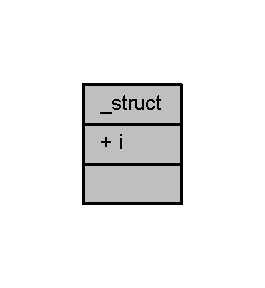
\includegraphics[width=127pt]{struct__struct__coll__graph}
\end{center}
\end{figure}
\subsection*{데이터 필드}
\begin{DoxyCompactItemize}
\item 
int \hyperlink{struct__struct_acb559820d9ca11295b4500f179ef6392}{i}
\end{DoxyCompactItemize}


\subsection{상세한 설명}


base.\+c 파일의 30 번째 라인에서 정의되었습니다.



\subsection{필드 문서화}
\mbox{\Hypertarget{struct__struct_acb559820d9ca11295b4500f179ef6392}\label{struct__struct_acb559820d9ca11295b4500f179ef6392}} 
\index{\+\_\+struct@{\+\_\+struct}!i@{i}}
\index{i@{i}!\+\_\+struct@{\+\_\+struct}}
\subsubsection{\texorpdfstring{i}{i}}
{\footnotesize\ttfamily int i}



base.\+c 파일의 31 번째 라인에서 정의되었습니다.



이 구조체에 대한 문서화 페이지는 다음의 파일들로부터 생성되었습니다.\+:\begin{DoxyCompactItemize}
\item 
src/function/\hyperlink{function_2base_8c}{base.\+c}\item 
src/keyword/\hyperlink{structure_8c}{structure.\+c}\item 
src/libstd/\hyperlink{abort_8c}{abort.\+c}\end{DoxyCompactItemize}

\hypertarget{structdata__st}{}\section{data\+\_\+st 구조체 참조}
\label{structdata__st}\index{data\+\_\+st@{data\+\_\+st}}


data\+\_\+st에 대한 협력 다이어그램\+:
\nopagebreak
\begin{figure}[H]
\begin{center}
\leavevmode
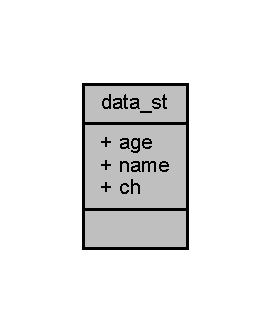
\includegraphics[width=130pt]{structdata__st__coll__graph}
\end{center}
\end{figure}
\subsection*{데이터 필드}
\begin{DoxyCompactItemize}
\item 
int32\+\_\+t \hyperlink{structdata__st_a63164120dd2834709fae48ecb4a9234e}{age}
\item 
int8\+\_\+t \hyperlink{structdata__st_aa6a4a36f30f93c1588dccd3030f66c37}{name} \mbox{[}25\mbox{]}
\item 
int8\+\_\+t \hyperlink{structdata__st_a6c669ea96fcb54a44ce1d6adf7969d80}{ch}
\end{DoxyCompactItemize}


\subsection{상세한 설명}


clock.\+c 파일의 30 번째 라인에서 정의되었습니다.



\subsection{필드 문서화}
\mbox{\Hypertarget{structdata__st_a63164120dd2834709fae48ecb4a9234e}\label{structdata__st_a63164120dd2834709fae48ecb4a9234e}} 
\index{data\+\_\+st@{data\+\_\+st}!age@{age}}
\index{age@{age}!data\+\_\+st@{data\+\_\+st}}
\subsubsection{\texorpdfstring{age}{age}}
{\footnotesize\ttfamily int32\+\_\+t age}



clock.\+c 파일의 31 번째 라인에서 정의되었습니다.

\mbox{\Hypertarget{structdata__st_a6c669ea96fcb54a44ce1d6adf7969d80}\label{structdata__st_a6c669ea96fcb54a44ce1d6adf7969d80}} 
\index{data\+\_\+st@{data\+\_\+st}!ch@{ch}}
\index{ch@{ch}!data\+\_\+st@{data\+\_\+st}}
\subsubsection{\texorpdfstring{ch}{ch}}
{\footnotesize\ttfamily int8\+\_\+t ch}



clock.\+c 파일의 33 번째 라인에서 정의되었습니다.

\mbox{\Hypertarget{structdata__st_aa6a4a36f30f93c1588dccd3030f66c37}\label{structdata__st_aa6a4a36f30f93c1588dccd3030f66c37}} 
\index{data\+\_\+st@{data\+\_\+st}!name@{name}}
\index{name@{name}!data\+\_\+st@{data\+\_\+st}}
\subsubsection{\texorpdfstring{name}{name}}
{\footnotesize\ttfamily int8\+\_\+t name\mbox{[}25\mbox{]}}



clock.\+c 파일의 32 번째 라인에서 정의되었습니다.



이 구조체에 대한 문서화 페이지는 다음의 파일로부터 생성되었습니다.\+:\begin{DoxyCompactItemize}
\item 
src/libstd/\hyperlink{clock_8c}{clock.\+c}\end{DoxyCompactItemize}

\hypertarget{structinventory}{}\section{inventory 구조체 참조}
\label{structinventory}\index{inventory@{inventory}}


inventory에 대한 협력 다이어그램\+:
\nopagebreak
\begin{figure}[H]
\begin{center}
\leavevmode
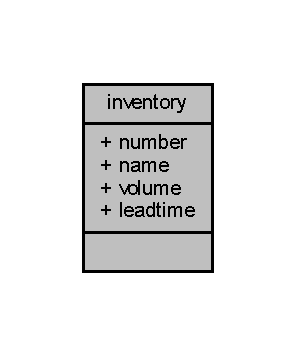
\includegraphics[width=142pt]{structinventory__coll__graph}
\end{center}
\end{figure}
\subsection*{데이터 필드}
\begin{DoxyCompactItemize}
\item 
char $\ast$ \hyperlink{structinventory_a77370bcefb3fe21e5f84e230581a50d7}{number}
\begin{DoxyCompactList}\small\item\em 상품 번호 \end{DoxyCompactList}\item 
char $\ast$ \hyperlink{structinventory_a5ac083a645d964373f022d03df4849c8}{name}
\begin{DoxyCompactList}\small\item\em 상품명 \end{DoxyCompactList}\item 
int \hyperlink{structinventory_aed48ca0bcd2162fd4fd495873e2631f5}{volume}
\begin{DoxyCompactList}\small\item\em 재고 수량 \end{DoxyCompactList}\item 
int \hyperlink{structinventory_ae0484109745ac918f2b3ed8551b41dcb}{leadtime}
\begin{DoxyCompactList}\small\item\em 매입 일수 \end{DoxyCompactList}\end{DoxyCompactItemize}


\subsection{상세한 설명}
상품 재고 관리용 inventory 구조체 정의 

main.\+c 파일의 31 번째 라인에서 정의되었습니다.



\subsection{필드 문서화}
\mbox{\Hypertarget{structinventory_ae0484109745ac918f2b3ed8551b41dcb}\label{structinventory_ae0484109745ac918f2b3ed8551b41dcb}} 
\index{inventory@{inventory}!leadtime@{leadtime}}
\index{leadtime@{leadtime}!inventory@{inventory}}
\subsubsection{\texorpdfstring{leadtime}{leadtime}}
{\footnotesize\ttfamily int leadtime}



매입 일수 



main.\+c 파일의 35 번째 라인에서 정의되었습니다.

\mbox{\Hypertarget{structinventory_a5ac083a645d964373f022d03df4849c8}\label{structinventory_a5ac083a645d964373f022d03df4849c8}} 
\index{inventory@{inventory}!name@{name}}
\index{name@{name}!inventory@{inventory}}
\subsubsection{\texorpdfstring{name}{name}}
{\footnotesize\ttfamily char$\ast$ name}



상품명 



main.\+c 파일의 33 번째 라인에서 정의되었습니다.

\mbox{\Hypertarget{structinventory_a77370bcefb3fe21e5f84e230581a50d7}\label{structinventory_a77370bcefb3fe21e5f84e230581a50d7}} 
\index{inventory@{inventory}!number@{number}}
\index{number@{number}!inventory@{inventory}}
\subsubsection{\texorpdfstring{number}{number}}
{\footnotesize\ttfamily char$\ast$ number}



상품 번호 



main.\+c 파일의 32 번째 라인에서 정의되었습니다.

\mbox{\Hypertarget{structinventory_aed48ca0bcd2162fd4fd495873e2631f5}\label{structinventory_aed48ca0bcd2162fd4fd495873e2631f5}} 
\index{inventory@{inventory}!volume@{volume}}
\index{volume@{volume}!inventory@{inventory}}
\subsubsection{\texorpdfstring{volume}{volume}}
{\footnotesize\ttfamily int volume}



재고 수량 



main.\+c 파일의 34 번째 라인에서 정의되었습니다.



이 구조체에 대한 문서화 페이지는 다음의 파일로부터 생성되었습니다.\+:\begin{DoxyCompactItemize}
\item 
src/function/\hyperlink{function_2main_8c}{main.\+c}\end{DoxyCompactItemize}

\chapter{파일 문서화}
\hypertarget{function_2base_8c}{}\section{src/function/base.c 파일 참조}
\label{function_2base_8c}\index{src/function/base.\+c@{src/function/base.\+c}}
{\ttfamily \#include $<$stdint.\+h$>$}\newline
{\ttfamily \#include $<$stdio.\+h$>$}\newline
{\ttfamily \#include $<$stddef.\+h$>$}\newline
{\ttfamily \#include $<$stdlib.\+h$>$}\newline
{\ttfamily \#include $<$string.\+h$>$}\newline
{\ttfamily \#include $<$stdarg.\+h$>$}\newline
{\ttfamily \#include $<$errno.\+h$>$}\newline
{\ttfamily \#include $<$assert.\+h$>$}\newline
{\ttfamily \#include $<$time.\+h$>$}\newline
base.\+c에 대한 include 의존 그래프
\nopagebreak
\begin{figure}[H]
\begin{center}
\leavevmode
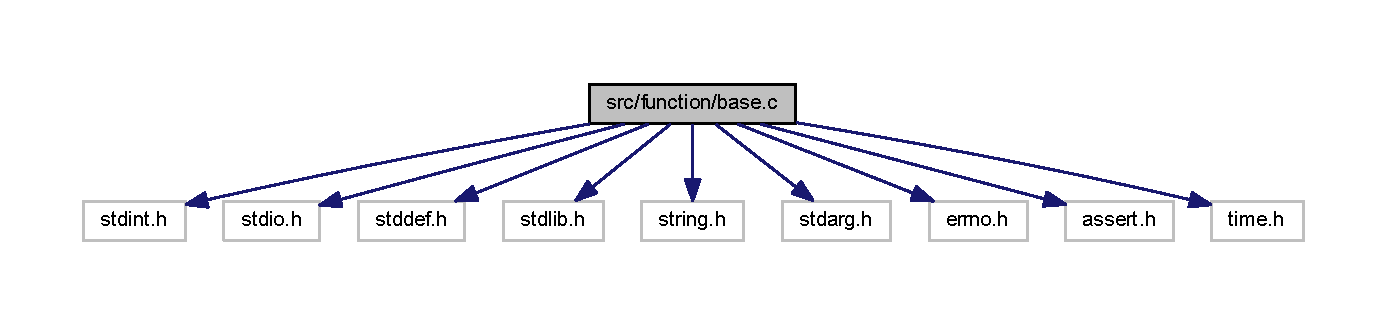
\includegraphics[width=350pt]{function_2base_8c__incl}
\end{center}
\end{figure}
\subsection*{데이터 구조}
\begin{DoxyCompactItemize}
\item 
struct \hyperlink{struct__struct}{\+\_\+struct}
\end{DoxyCompactItemize}
\subsection*{매크로}
\begin{DoxyCompactItemize}
\item 
\#define \hyperlink{function_2base_8c_a6c7cd32e1bac137f05e4a752b4ad10af}{B\+U\+F\+F\+\_\+\+S\+I\+ZE}~256
\begin{DoxyCompactList}\small\item\em Buffer size for character data \end{DoxyCompactList}\end{DoxyCompactItemize}
\subsection*{타입정의}
\begin{DoxyCompactItemize}
\item 
typedef struct \hyperlink{struct__struct}{\+\_\+struct} \hyperlink{function_2base_8c_a6a0147790bea2d2ab884eaf27ce874d1}{S\+T\+R\+U\+CT}
\end{DoxyCompactItemize}
\subsection*{함수}
\begin{DoxyCompactItemize}
\item 
int \hyperlink{function_2base_8c_abf9e6b7e6f15df4b525a2e7705ba3089}{main} (int argc, char const $\ast$argv\mbox{[}$\,$\mbox{]})
\end{DoxyCompactItemize}


\subsection{상세한 설명}
\begin{DoxyAuthor}{작성자}

\end{DoxyAuthor}
\begin{DoxyDate}{날짜}

\end{DoxyDate}
\begin{DoxySeeAlso}{참고}

\end{DoxySeeAlso}


\subsection{매크로 문서화}
\mbox{\Hypertarget{function_2base_8c_a6c7cd32e1bac137f05e4a752b4ad10af}\label{function_2base_8c_a6c7cd32e1bac137f05e4a752b4ad10af}} 
\index{function/base.\+c@{function/base.\+c}!B\+U\+F\+F\+\_\+\+S\+I\+ZE@{B\+U\+F\+F\+\_\+\+S\+I\+ZE}}
\index{B\+U\+F\+F\+\_\+\+S\+I\+ZE@{B\+U\+F\+F\+\_\+\+S\+I\+ZE}!function/base.\+c@{function/base.\+c}}
\subsubsection{\texorpdfstring{B\+U\+F\+F\+\_\+\+S\+I\+ZE}{BUFF\_SIZE}}
{\footnotesize\ttfamily \#define B\+U\+F\+F\+\_\+\+S\+I\+ZE~256}



Buffer size for character data 



base.\+c 파일의 22 번째 라인에서 정의되었습니다.



\subsection{타입정의 문서화}
\mbox{\Hypertarget{function_2base_8c_a6a0147790bea2d2ab884eaf27ce874d1}\label{function_2base_8c_a6a0147790bea2d2ab884eaf27ce874d1}} 
\index{function/base.\+c@{function/base.\+c}!S\+T\+R\+U\+CT@{S\+T\+R\+U\+CT}}
\index{S\+T\+R\+U\+CT@{S\+T\+R\+U\+CT}!function/base.\+c@{function/base.\+c}}
\subsubsection{\texorpdfstring{S\+T\+R\+U\+CT}{STRUCT}}
{\footnotesize\ttfamily typedef struct \hyperlink{struct__struct}{\+\_\+struct}  \hyperlink{function_2base_8c_a6a0147790bea2d2ab884eaf27ce874d1}{S\+T\+R\+U\+CT}}



\subsection{함수 문서화}
\mbox{\Hypertarget{function_2base_8c_abf9e6b7e6f15df4b525a2e7705ba3089}\label{function_2base_8c_abf9e6b7e6f15df4b525a2e7705ba3089}} 
\index{function/base.\+c@{function/base.\+c}!main@{main}}
\index{main@{main}!function/base.\+c@{function/base.\+c}}
\subsubsection{\texorpdfstring{main()}{main()}}
{\footnotesize\ttfamily int main (\begin{DoxyParamCaption}\item[{int}]{argc,  }\item[{char const $\ast$}]{argv\mbox{[}$\,$\mbox{]} }\end{DoxyParamCaption})}



base.\+c 파일의 54 번째 라인에서 정의되었습니다.


\begin{DoxyCode}
54                                        \{
55   
56   \textcolor{keywordflow}{return} 0;
57 \}
\end{DoxyCode}

\hypertarget{libstd_2base_8c}{}\section{src/libstd/base.c 파일 참조}
\label{libstd_2base_8c}\index{src/libstd/base.\+c@{src/libstd/base.\+c}}
{\ttfamily \#include $<$stdint.\+h$>$}\newline
{\ttfamily \#include $<$stdio.\+h$>$}\newline
{\ttfamily \#include $<$stddef.\+h$>$}\newline
{\ttfamily \#include $<$stdlib.\+h$>$}\newline
{\ttfamily \#include $<$string.\+h$>$}\newline
{\ttfamily \#include $<$stdarg.\+h$>$}\newline
{\ttfamily \#include $<$errno.\+h$>$}\newline
{\ttfamily \#include $<$assert.\+h$>$}\newline
{\ttfamily \#include $<$time.\+h$>$}\newline
base.\+c에 대한 include 의존 그래프
\nopagebreak
\begin{figure}[H]
\begin{center}
\leavevmode
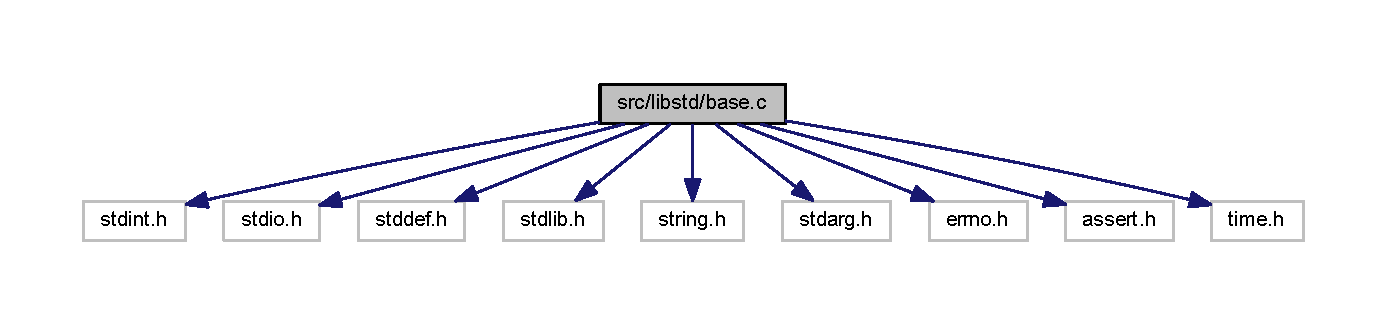
\includegraphics[width=350pt]{libstd_2base_8c__incl}
\end{center}
\end{figure}
\subsection*{데이터 구조}
\begin{DoxyCompactItemize}
\item 
struct \hyperlink{struct__struct}{\+\_\+struct}
\end{DoxyCompactItemize}
\subsection*{매크로}
\begin{DoxyCompactItemize}
\item 
\#define \hyperlink{libstd_2base_8c_a6c7cd32e1bac137f05e4a752b4ad10af}{B\+U\+F\+F\+\_\+\+S\+I\+ZE}~256
\begin{DoxyCompactList}\small\item\em Buffer size for character data \end{DoxyCompactList}\end{DoxyCompactItemize}
\subsection*{타입정의}
\begin{DoxyCompactItemize}
\item 
typedef struct \hyperlink{struct__struct}{\+\_\+struct} \hyperlink{libstd_2base_8c_a6a0147790bea2d2ab884eaf27ce874d1}{S\+T\+R\+U\+CT}
\end{DoxyCompactItemize}
\subsection*{함수}
\begin{DoxyCompactItemize}
\item 
int \hyperlink{libstd_2base_8c_abf9e6b7e6f15df4b525a2e7705ba3089}{main} (int argc, char const $\ast$argv\mbox{[}$\,$\mbox{]})
\end{DoxyCompactItemize}


\subsection{상세한 설명}
\begin{DoxyAuthor}{작성자}

\end{DoxyAuthor}
\begin{DoxyDate}{날짜}

\end{DoxyDate}
\begin{DoxySeeAlso}{참고}

\end{DoxySeeAlso}


\subsection{매크로 문서화}
\mbox{\Hypertarget{libstd_2base_8c_a6c7cd32e1bac137f05e4a752b4ad10af}\label{libstd_2base_8c_a6c7cd32e1bac137f05e4a752b4ad10af}} 
\index{libstd/base.\+c@{libstd/base.\+c}!B\+U\+F\+F\+\_\+\+S\+I\+ZE@{B\+U\+F\+F\+\_\+\+S\+I\+ZE}}
\index{B\+U\+F\+F\+\_\+\+S\+I\+ZE@{B\+U\+F\+F\+\_\+\+S\+I\+ZE}!libstd/base.\+c@{libstd/base.\+c}}
\subsubsection{\texorpdfstring{B\+U\+F\+F\+\_\+\+S\+I\+ZE}{BUFF\_SIZE}}
{\footnotesize\ttfamily \#define B\+U\+F\+F\+\_\+\+S\+I\+ZE~256}



Buffer size for character data 



base.\+c 파일의 22 번째 라인에서 정의되었습니다.



\subsection{타입정의 문서화}
\mbox{\Hypertarget{libstd_2base_8c_a6a0147790bea2d2ab884eaf27ce874d1}\label{libstd_2base_8c_a6a0147790bea2d2ab884eaf27ce874d1}} 
\index{libstd/base.\+c@{libstd/base.\+c}!S\+T\+R\+U\+CT@{S\+T\+R\+U\+CT}}
\index{S\+T\+R\+U\+CT@{S\+T\+R\+U\+CT}!libstd/base.\+c@{libstd/base.\+c}}
\subsubsection{\texorpdfstring{S\+T\+R\+U\+CT}{STRUCT}}
{\footnotesize\ttfamily typedef struct \hyperlink{struct__struct}{\+\_\+struct}  \hyperlink{function_2base_8c_a6a0147790bea2d2ab884eaf27ce874d1}{S\+T\+R\+U\+CT}}



\subsection{함수 문서화}
\mbox{\Hypertarget{libstd_2base_8c_abf9e6b7e6f15df4b525a2e7705ba3089}\label{libstd_2base_8c_abf9e6b7e6f15df4b525a2e7705ba3089}} 
\index{libstd/base.\+c@{libstd/base.\+c}!main@{main}}
\index{main@{main}!libstd/base.\+c@{libstd/base.\+c}}
\subsubsection{\texorpdfstring{main()}{main()}}
{\footnotesize\ttfamily int main (\begin{DoxyParamCaption}\item[{int}]{argc,  }\item[{char const $\ast$}]{argv\mbox{[}$\,$\mbox{]} }\end{DoxyParamCaption})}



base.\+c 파일의 54 번째 라인에서 정의되었습니다.


\begin{DoxyCode}
54                                        \{
55   
56   \textcolor{keywordflow}{return} 0;
57 \}
\end{DoxyCode}

\hypertarget{_declaring___attributes__of___functions_8c}{}\section{src/function/\+Declaring\+\_\+\+Attributes\+\_\+of\+\_\+\+Functions.c 파일 참조}
\label{_declaring___attributes__of___functions_8c}\index{src/function/\+Declaring\+\_\+\+Attributes\+\_\+of\+\_\+\+Functions.\+c@{src/function/\+Declaring\+\_\+\+Attributes\+\_\+of\+\_\+\+Functions.\+c}}
{\ttfamily \#include $<$stdio.\+h$>$}\newline
{\ttfamily \#include $<$stdarg.\+h$>$}\newline
{\ttfamily \#include $<$stdlib.\+h$>$}\newline
{\ttfamily \#include $<$linux/types.\+h$>$}\newline
{\ttfamily \#include \char`\"{}Declaring\+\_\+\+Attributes\+\_\+of\+\_\+\+Functions.\+h\char`\"{}}\newline
Declaring\+\_\+\+Attributes\+\_\+of\+\_\+\+Functions.\+c에 대한 include 의존 그래프
\nopagebreak
\begin{figure}[H]
\begin{center}
\leavevmode
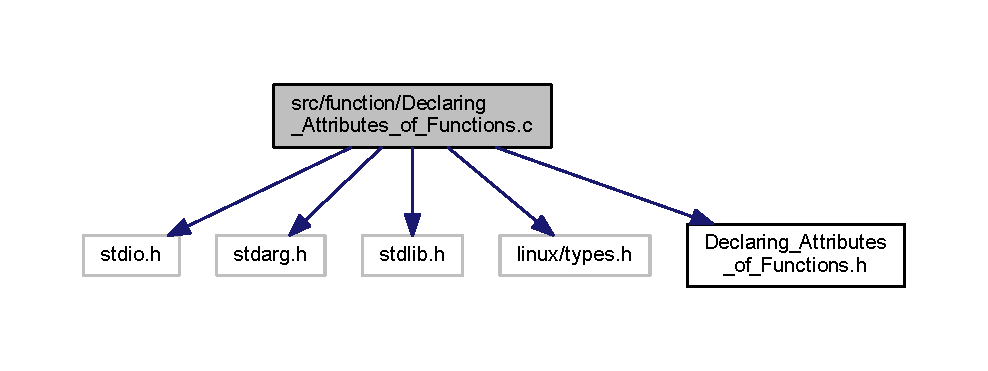
\includegraphics[width=350pt]{_declaring___attributes__of___functions_8c__incl}
\end{center}
\end{figure}
\subsection*{함수}
\begin{DoxyCompactItemize}
\item 
void \hyperlink{_declaring___attributes__of___functions_8c_a1030d865f310a3bd612e70abcead89f1}{\+\_\+\+\_\+func\+\_\+noreturn} (void)
\item 
void \hyperlink{_declaring___attributes__of___functions_8c_ad3c2e96589683757ac6d263dc4d68753}{f\+\_\+noreturn} (void)
\item 
void \hyperlink{_declaring___attributes__of___functions_8c_ae4dd766abad745c5113303b9ea06c8de}{f\+\_\+nonnull} (void $\ast$dest, const void $\ast$src, size\+\_\+t len) \+\_\+\+\_\+attribute\+\_\+\+\_\+((weak
\item 
void \hyperlink{_declaring___attributes__of___functions_8c_a640d88ac74f57e25b1b6d813744c5f54}{alias} (\char`\"{}\+\_\+\+\_\+func\+\_\+nonnull\char`\"{})))
\item 
void \hyperlink{_declaring___attributes__of___functions_8c_a4db90b53c3f6e50011916a36a4905bee}{\+\_\+\+\_\+func\+\_\+visibility} (void)
\item 
void \hyperlink{_declaring___attributes__of___functions_8c_afc4e2b93731b1fcae62fe25d5c3a9fd1}{f\+\_\+visibility} (void)
\item 
int \hyperlink{_declaring___attributes__of___functions_8c_af7e19d11f45bdef39e05946fa24aafd0}{f\+\_\+warn\+\_\+unused\+\_\+result} (void)
\item 
void \hyperlink{_declaring___attributes__of___functions_8c_af729a5eb32486892390961ab15e017f0}{f\+\_\+weakref} (void)
\item 
void \hyperlink{_declaring___attributes__of___functions_8c_a677a2f44d0dc12217eb3ccbbc623f8ba}{debug} (\+\_\+\+\_\+s32 dlevel, const char $\ast$fmt,...)
\end{DoxyCompactItemize}


\subsection{함수 문서화}
\mbox{\Hypertarget{_declaring___attributes__of___functions_8c_a1030d865f310a3bd612e70abcead89f1}\label{_declaring___attributes__of___functions_8c_a1030d865f310a3bd612e70abcead89f1}} 
\index{Declaring\+\_\+\+Attributes\+\_\+of\+\_\+\+Functions.\+c@{Declaring\+\_\+\+Attributes\+\_\+of\+\_\+\+Functions.\+c}!\+\_\+\+\_\+func\+\_\+noreturn@{\+\_\+\+\_\+func\+\_\+noreturn}}
\index{\+\_\+\+\_\+func\+\_\+noreturn@{\+\_\+\+\_\+func\+\_\+noreturn}!Declaring\+\_\+\+Attributes\+\_\+of\+\_\+\+Functions.\+c@{Declaring\+\_\+\+Attributes\+\_\+of\+\_\+\+Functions.\+c}}
\subsubsection{\texorpdfstring{\+\_\+\+\_\+func\+\_\+noreturn()}{\_\_func\_noreturn()}}
{\footnotesize\ttfamily void \+\_\+\+\_\+func\+\_\+noreturn (\begin{DoxyParamCaption}\item[{void}]{ }\end{DoxyParamCaption})}



Declaring\+\_\+\+Attributes\+\_\+of\+\_\+\+Functions.\+c 파일의 7 번째 라인에서 정의되었습니다.


\begin{DoxyCode}
8 \{
9     \hyperlink{_declaring___attributes__of___functions_8c_a677a2f44d0dc12217eb3ccbbc623f8ba}{debug}(1, \textcolor{stringliteral}{"%s is called..\(\backslash\)n"}, \_\_func\_\_);
10     exit(1); \textcolor{comment}{/* or abort(); */}
11 \}
\end{DoxyCode}
이 함수 내부에서 호출하는 함수들에 대한 그래프입니다.\+:
\nopagebreak
\begin{figure}[H]
\begin{center}
\leavevmode
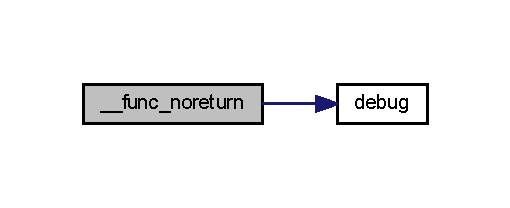
\includegraphics[width=245pt]{_declaring___attributes__of___functions_8c_a1030d865f310a3bd612e70abcead89f1_cgraph}
\end{center}
\end{figure}
\mbox{\Hypertarget{_declaring___attributes__of___functions_8c_a4db90b53c3f6e50011916a36a4905bee}\label{_declaring___attributes__of___functions_8c_a4db90b53c3f6e50011916a36a4905bee}} 
\index{Declaring\+\_\+\+Attributes\+\_\+of\+\_\+\+Functions.\+c@{Declaring\+\_\+\+Attributes\+\_\+of\+\_\+\+Functions.\+c}!\+\_\+\+\_\+func\+\_\+visibility@{\+\_\+\+\_\+func\+\_\+visibility}}
\index{\+\_\+\+\_\+func\+\_\+visibility@{\+\_\+\+\_\+func\+\_\+visibility}!Declaring\+\_\+\+Attributes\+\_\+of\+\_\+\+Functions.\+c@{Declaring\+\_\+\+Attributes\+\_\+of\+\_\+\+Functions.\+c}}
\subsubsection{\texorpdfstring{\+\_\+\+\_\+func\+\_\+visibility()}{\_\_func\_visibility()}}
{\footnotesize\ttfamily void \+\_\+\+\_\+func\+\_\+visibility (\begin{DoxyParamCaption}\item[{void}]{ }\end{DoxyParamCaption})}



Declaring\+\_\+\+Attributes\+\_\+of\+\_\+\+Functions.\+c 파일의 22 번째 라인에서 정의되었습니다.


\begin{DoxyCode}
23 \{
24     \hyperlink{_declaring___attributes__of___functions_8c_a677a2f44d0dc12217eb3ccbbc623f8ba}{debug}(1, \textcolor{stringliteral}{"%s is called..\(\backslash\)n"}, \_\_func\_\_);
25 \}
\end{DoxyCode}
이 함수 내부에서 호출하는 함수들에 대한 그래프입니다.\+:
\nopagebreak
\begin{figure}[H]
\begin{center}
\leavevmode
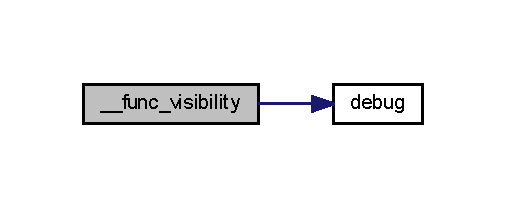
\includegraphics[width=243pt]{_declaring___attributes__of___functions_8c_a4db90b53c3f6e50011916a36a4905bee_cgraph}
\end{center}
\end{figure}
\mbox{\Hypertarget{_declaring___attributes__of___functions_8c_a640d88ac74f57e25b1b6d813744c5f54}\label{_declaring___attributes__of___functions_8c_a640d88ac74f57e25b1b6d813744c5f54}} 
\index{Declaring\+\_\+\+Attributes\+\_\+of\+\_\+\+Functions.\+c@{Declaring\+\_\+\+Attributes\+\_\+of\+\_\+\+Functions.\+c}!alias@{alias}}
\index{alias@{alias}!Declaring\+\_\+\+Attributes\+\_\+of\+\_\+\+Functions.\+c@{Declaring\+\_\+\+Attributes\+\_\+of\+\_\+\+Functions.\+c}}
\subsubsection{\texorpdfstring{alias()}{alias()}}
{\footnotesize\ttfamily void alias (\begin{DoxyParamCaption}\item[{\char`\"{}\+\_\+\+\_\+func\+\_\+nonnull\char`\"{}}]{ }\end{DoxyParamCaption})}

\mbox{\Hypertarget{_declaring___attributes__of___functions_8c_a677a2f44d0dc12217eb3ccbbc623f8ba}\label{_declaring___attributes__of___functions_8c_a677a2f44d0dc12217eb3ccbbc623f8ba}} 
\index{Declaring\+\_\+\+Attributes\+\_\+of\+\_\+\+Functions.\+c@{Declaring\+\_\+\+Attributes\+\_\+of\+\_\+\+Functions.\+c}!debug@{debug}}
\index{debug@{debug}!Declaring\+\_\+\+Attributes\+\_\+of\+\_\+\+Functions.\+c@{Declaring\+\_\+\+Attributes\+\_\+of\+\_\+\+Functions.\+c}}
\subsubsection{\texorpdfstring{debug()}{debug()}}
{\footnotesize\ttfamily void debug (\begin{DoxyParamCaption}\item[{\+\_\+\+\_\+s32}]{dlevel,  }\item[{const char $\ast$}]{fmt,  }\item[{}]{... }\end{DoxyParamCaption})}



Declaring\+\_\+\+Attributes\+\_\+of\+\_\+\+Functions.\+c 파일의 53 번째 라인에서 정의되었습니다.


\begin{DoxyCode}
54 \{
55     va\_list ap;
56     va\_start (ap, fmt);
57 
58     \textcolor{keywordflow}{switch} (dlevel) \{
59     \textcolor{keywordflow}{case} 0:
60         \textcolor{keywordflow}{break};
61     \textcolor{keywordflow}{case} 1:
62         vfprintf(stdout, fmt, ap);
63         va\_end(ap);
64         \textcolor{keywordflow}{break};
65     \textcolor{keywordflow}{default}:
66         vfprintf(stdout, fmt, ap);
67         va\_end(ap);
68         \textcolor{keywordflow}{break};
69     \};
70 \}
\end{DoxyCode}
이 함수를 호출하는 함수들에 대한 그래프입니다.\+:
\nopagebreak
\begin{figure}[H]
\begin{center}
\leavevmode
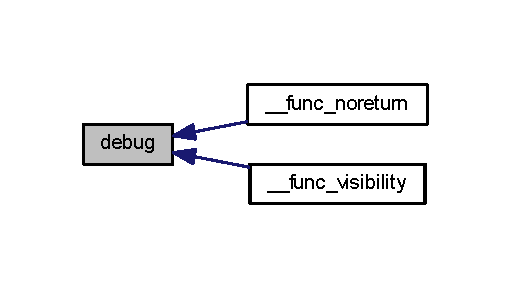
\includegraphics[width=245pt]{_declaring___attributes__of___functions_8c_a677a2f44d0dc12217eb3ccbbc623f8ba_icgraph}
\end{center}
\end{figure}
\mbox{\Hypertarget{_declaring___attributes__of___functions_8c_ae4dd766abad745c5113303b9ea06c8de}\label{_declaring___attributes__of___functions_8c_ae4dd766abad745c5113303b9ea06c8de}} 
\index{Declaring\+\_\+\+Attributes\+\_\+of\+\_\+\+Functions.\+c@{Declaring\+\_\+\+Attributes\+\_\+of\+\_\+\+Functions.\+c}!f\+\_\+nonnull@{f\+\_\+nonnull}}
\index{f\+\_\+nonnull@{f\+\_\+nonnull}!Declaring\+\_\+\+Attributes\+\_\+of\+\_\+\+Functions.\+c@{Declaring\+\_\+\+Attributes\+\_\+of\+\_\+\+Functions.\+c}}
\subsubsection{\texorpdfstring{f\+\_\+nonnull()}{f\_nonnull()}}
{\footnotesize\ttfamily void f\+\_\+nonnull (\begin{DoxyParamCaption}\item[{void $\ast$}]{dest,  }\item[{const void $\ast$}]{src,  }\item[{size\+\_\+t}]{len }\end{DoxyParamCaption})}

\mbox{\Hypertarget{_declaring___attributes__of___functions_8c_ad3c2e96589683757ac6d263dc4d68753}\label{_declaring___attributes__of___functions_8c_ad3c2e96589683757ac6d263dc4d68753}} 
\index{Declaring\+\_\+\+Attributes\+\_\+of\+\_\+\+Functions.\+c@{Declaring\+\_\+\+Attributes\+\_\+of\+\_\+\+Functions.\+c}!f\+\_\+noreturn@{f\+\_\+noreturn}}
\index{f\+\_\+noreturn@{f\+\_\+noreturn}!Declaring\+\_\+\+Attributes\+\_\+of\+\_\+\+Functions.\+c@{Declaring\+\_\+\+Attributes\+\_\+of\+\_\+\+Functions.\+c}}
\subsubsection{\texorpdfstring{f\+\_\+noreturn()}{f\_noreturn()}}
{\footnotesize\ttfamily void f\+\_\+noreturn (\begin{DoxyParamCaption}\item[{void}]{ }\end{DoxyParamCaption})}



Declaring\+\_\+\+Attributes\+\_\+of\+\_\+\+Functions.\+c 파일의 13 번째 라인에서 정의되었습니다.


\begin{DoxyCode}
16 \{
17     \hyperlink{_declaring___attributes__of___functions_8c_a677a2f44d0dc12217eb3ccbbc623f8ba}{debug}(1, \textcolor{stringliteral}{"%s is called..\(\backslash\)n"}, \_\_func\_\_);
18 \}
\end{DoxyCode}
\mbox{\Hypertarget{_declaring___attributes__of___functions_8c_afc4e2b93731b1fcae62fe25d5c3a9fd1}\label{_declaring___attributes__of___functions_8c_afc4e2b93731b1fcae62fe25d5c3a9fd1}} 
\index{Declaring\+\_\+\+Attributes\+\_\+of\+\_\+\+Functions.\+c@{Declaring\+\_\+\+Attributes\+\_\+of\+\_\+\+Functions.\+c}!f\+\_\+visibility@{f\+\_\+visibility}}
\index{f\+\_\+visibility@{f\+\_\+visibility}!Declaring\+\_\+\+Attributes\+\_\+of\+\_\+\+Functions.\+c@{Declaring\+\_\+\+Attributes\+\_\+of\+\_\+\+Functions.\+c}}
\subsubsection{\texorpdfstring{f\+\_\+visibility()}{f\_visibility()}}
{\footnotesize\ttfamily void f\+\_\+visibility (\begin{DoxyParamCaption}\item[{void}]{ }\end{DoxyParamCaption})}



Declaring\+\_\+\+Attributes\+\_\+of\+\_\+\+Functions.\+c 파일의 27 번째 라인에서 정의되었습니다.


\begin{DoxyCode}
31 \{
32     \hyperlink{_declaring___attributes__of___functions_8c_a677a2f44d0dc12217eb3ccbbc623f8ba}{debug}(1, \textcolor{stringliteral}{"%s is called..\(\backslash\)n"}, \_\_func\_\_);
33     \textcolor{keywordflow}{return} 0;
34 \}
\end{DoxyCode}
\mbox{\Hypertarget{_declaring___attributes__of___functions_8c_af7e19d11f45bdef39e05946fa24aafd0}\label{_declaring___attributes__of___functions_8c_af7e19d11f45bdef39e05946fa24aafd0}} 
\index{Declaring\+\_\+\+Attributes\+\_\+of\+\_\+\+Functions.\+c@{Declaring\+\_\+\+Attributes\+\_\+of\+\_\+\+Functions.\+c}!f\+\_\+warn\+\_\+unused\+\_\+result@{f\+\_\+warn\+\_\+unused\+\_\+result}}
\index{f\+\_\+warn\+\_\+unused\+\_\+result@{f\+\_\+warn\+\_\+unused\+\_\+result}!Declaring\+\_\+\+Attributes\+\_\+of\+\_\+\+Functions.\+c@{Declaring\+\_\+\+Attributes\+\_\+of\+\_\+\+Functions.\+c}}
\subsubsection{\texorpdfstring{f\+\_\+warn\+\_\+unused\+\_\+result()}{f\_warn\_unused\_result()}}
{\footnotesize\ttfamily int f\+\_\+warn\+\_\+unused\+\_\+result (\begin{DoxyParamCaption}\item[{void}]{ }\end{DoxyParamCaption})}



Declaring\+\_\+\+Attributes\+\_\+of\+\_\+\+Functions.\+c 파일의 36 번째 라인에서 정의되었습니다.


\begin{DoxyCode}
39 \{
40     \hyperlink{_declaring___attributes__of___functions_8c_a677a2f44d0dc12217eb3ccbbc623f8ba}{debug}(1, \textcolor{stringliteral}{"%s is called..\(\backslash\)n"}, \_\_func\_\_);
41 \}
\end{DoxyCode}
\mbox{\Hypertarget{_declaring___attributes__of___functions_8c_af729a5eb32486892390961ab15e017f0}\label{_declaring___attributes__of___functions_8c_af729a5eb32486892390961ab15e017f0}} 
\index{Declaring\+\_\+\+Attributes\+\_\+of\+\_\+\+Functions.\+c@{Declaring\+\_\+\+Attributes\+\_\+of\+\_\+\+Functions.\+c}!f\+\_\+weakref@{f\+\_\+weakref}}
\index{f\+\_\+weakref@{f\+\_\+weakref}!Declaring\+\_\+\+Attributes\+\_\+of\+\_\+\+Functions.\+c@{Declaring\+\_\+\+Attributes\+\_\+of\+\_\+\+Functions.\+c}}
\subsubsection{\texorpdfstring{f\+\_\+weakref()}{f\_weakref()}}
{\footnotesize\ttfamily void f\+\_\+weakref (\begin{DoxyParamCaption}\item[{void}]{ }\end{DoxyParamCaption})}



Declaring\+\_\+\+Attributes\+\_\+of\+\_\+\+Functions.\+c 파일의 42 번째 라인에서 정의되었습니다.


\begin{DoxyCode}
45 \{
46     va\_list ap;
47     va\_start (ap, fmt);
48 
49     vfprintf(stderr, fmt, ap);
50     va\_end(ap);   
51 \}
\end{DoxyCode}

\hypertarget{_declaring___attributes__of___functions_8h}{}\section{src/function/\+Declaring\+\_\+\+Attributes\+\_\+of\+\_\+\+Functions.h 파일 참조}
\label{_declaring___attributes__of___functions_8h}\index{src/function/\+Declaring\+\_\+\+Attributes\+\_\+of\+\_\+\+Functions.\+h@{src/function/\+Declaring\+\_\+\+Attributes\+\_\+of\+\_\+\+Functions.\+h}}
이 그래프는 이 파일을 직/간접적으로 include 하는 파일들을 보여줍니다.\+:
\nopagebreak
\begin{figure}[H]
\begin{center}
\leavevmode
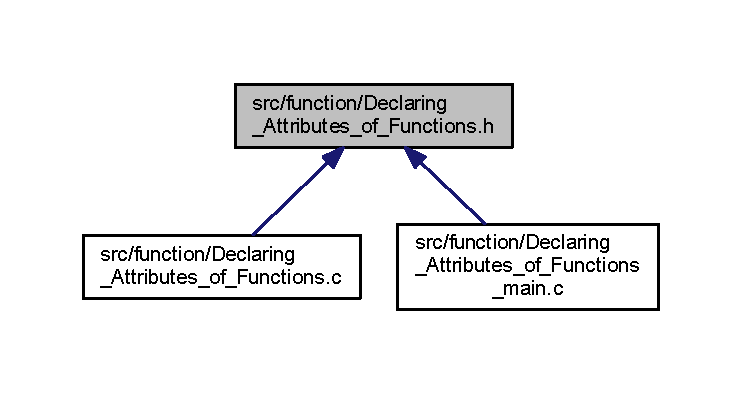
\includegraphics[width=350pt]{_declaring___attributes__of___functions_8h__dep__incl}
\end{center}
\end{figure}
\subsection*{함수}
\begin{DoxyCompactItemize}
\item 
void \hyperlink{_declaring___attributes__of___functions_8h_a2f9582bef5dfe15aab08367e45e02a3f}{f\+\_\+noreturn} (void) \+\_\+\+\_\+attribute\+\_\+\+\_\+((noreturn))
\item 
void \hyperlink{_declaring___attributes__of___functions_8h_ace09e9735ddb34c9cf9e6de2ebb2be49}{f\+\_\+nonnull} (void $\ast$dest, const void $\ast$src, size\+\_\+t len) \+\_\+\+\_\+attribute\+\_\+\+\_\+((nonnull))
\item 
void \hyperlink{_declaring___attributes__of___functions_8h_a1a2fc7e33ab06ba46dc47f7c63c3f60e}{f\+\_\+visibility} (void) \+\_\+\+\_\+attribute\+\_\+\+\_\+((visibility(\char`\"{}hidden\char`\"{})))
\item 
int \hyperlink{_declaring___attributes__of___functions_8h_a53dea1426a2c6d2c6f792cbc78aacc96}{f\+\_\+warn\+\_\+unused\+\_\+result} (void) \+\_\+\+\_\+attribute\+\_\+\+\_\+((warn\+\_\+unused\+\_\+result))
\item 
void \hyperlink{_declaring___attributes__of___functions_8h_af729a5eb32486892390961ab15e017f0}{f\+\_\+weakref} (void)
\item 
void \hyperlink{_declaring___attributes__of___functions_8h_ac9e09fe63e9ed7a03260bdbc2c2eadaf}{\+\_\+\+\_\+func\+\_\+noreturn} (void) \+\_\+\+\_\+attribute\+\_\+\+\_\+((noreturn))
\item 
void \hyperlink{_declaring___attributes__of___functions_8h_aa75bbbcbd03048e53258628904a94585}{\+\_\+\+\_\+func\+\_\+nonnull} (void $\ast$dest, const void $\ast$src, size\+\_\+t len) \+\_\+\+\_\+attribute\+\_\+\+\_\+((nonnull))
\item 
void \hyperlink{_declaring___attributes__of___functions_8h_a6307cb225a3697c3c667e46fb27c3a74}{\+\_\+\+\_\+func\+\_\+visibility} (void) \+\_\+\+\_\+attribute\+\_\+\+\_\+((visibility(\char`\"{}hidden\char`\"{})))
\item 
int \hyperlink{_declaring___attributes__of___functions_8h_a1b1e21f7bd1cc25b71a72304b05004cd}{\+\_\+\+\_\+func\+\_\+warn\+\_\+unused\+\_\+result} (void) \+\_\+\+\_\+attribute\+\_\+\+\_\+((warn\+\_\+unused\+\_\+result))
\item 
void \hyperlink{_declaring___attributes__of___functions_8h_ab057dfa6daeabaf2388048dc18b5a794}{\+\_\+\+\_\+func\+\_\+weakref} (void)
\item 
void \hyperlink{_declaring___attributes__of___functions_8h_ad8bf4027913439e0459739896645d771}{error} (const char $\ast$format,...) \+\_\+\+\_\+attribute\+\_\+\+\_\+((format(printf
\item 
void void \hyperlink{_declaring___attributes__of___functions_8h_a8f556a5a59e1162e11b05baec39ee3f9}{debug} (int dlevel, const char $\ast$format,...) \+\_\+\+\_\+attribute\+\_\+\+\_\+((format(printf
\end{DoxyCompactItemize}


\subsection{함수 문서화}
\mbox{\Hypertarget{_declaring___attributes__of___functions_8h_aa75bbbcbd03048e53258628904a94585}\label{_declaring___attributes__of___functions_8h_aa75bbbcbd03048e53258628904a94585}} 
\index{Declaring\+\_\+\+Attributes\+\_\+of\+\_\+\+Functions.\+h@{Declaring\+\_\+\+Attributes\+\_\+of\+\_\+\+Functions.\+h}!\+\_\+\+\_\+func\+\_\+nonnull@{\+\_\+\+\_\+func\+\_\+nonnull}}
\index{\+\_\+\+\_\+func\+\_\+nonnull@{\+\_\+\+\_\+func\+\_\+nonnull}!Declaring\+\_\+\+Attributes\+\_\+of\+\_\+\+Functions.\+h@{Declaring\+\_\+\+Attributes\+\_\+of\+\_\+\+Functions.\+h}}
\subsubsection{\texorpdfstring{\+\_\+\+\_\+func\+\_\+nonnull()}{\_\_func\_nonnull()}}
{\footnotesize\ttfamily void \+\_\+\+\_\+func\+\_\+nonnull (\begin{DoxyParamCaption}\item[{void $\ast$}]{dest,  }\item[{const void $\ast$}]{src,  }\item[{size\+\_\+t}]{len }\end{DoxyParamCaption})}

\mbox{\Hypertarget{_declaring___attributes__of___functions_8h_ac9e09fe63e9ed7a03260bdbc2c2eadaf}\label{_declaring___attributes__of___functions_8h_ac9e09fe63e9ed7a03260bdbc2c2eadaf}} 
\index{Declaring\+\_\+\+Attributes\+\_\+of\+\_\+\+Functions.\+h@{Declaring\+\_\+\+Attributes\+\_\+of\+\_\+\+Functions.\+h}!\+\_\+\+\_\+func\+\_\+noreturn@{\+\_\+\+\_\+func\+\_\+noreturn}}
\index{\+\_\+\+\_\+func\+\_\+noreturn@{\+\_\+\+\_\+func\+\_\+noreturn}!Declaring\+\_\+\+Attributes\+\_\+of\+\_\+\+Functions.\+h@{Declaring\+\_\+\+Attributes\+\_\+of\+\_\+\+Functions.\+h}}
\subsubsection{\texorpdfstring{\+\_\+\+\_\+func\+\_\+noreturn()}{\_\_func\_noreturn()}}
{\footnotesize\ttfamily void \+\_\+\+\_\+func\+\_\+noreturn (\begin{DoxyParamCaption}\item[{void}]{ }\end{DoxyParamCaption})}



Declaring\+\_\+\+Attributes\+\_\+of\+\_\+\+Functions.\+c 파일의 7 번째 라인에서 정의되었습니다.


\begin{DoxyCode}
8 \{
9     \hyperlink{_declaring___attributes__of___functions_8c_a677a2f44d0dc12217eb3ccbbc623f8ba}{debug}(1, \textcolor{stringliteral}{"%s is called..\(\backslash\)n"}, \_\_func\_\_);
10     exit(1); \textcolor{comment}{/* or abort(); */}
11 \}
\end{DoxyCode}
이 함수 내부에서 호출하는 함수들에 대한 그래프입니다.\+:
\nopagebreak
\begin{figure}[H]
\begin{center}
\leavevmode
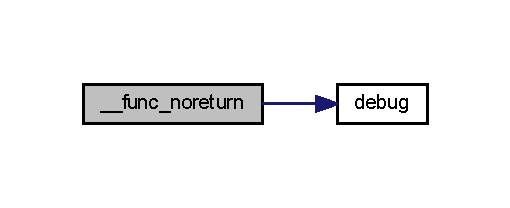
\includegraphics[width=245pt]{_declaring___attributes__of___functions_8h_ac9e09fe63e9ed7a03260bdbc2c2eadaf_cgraph}
\end{center}
\end{figure}
\mbox{\Hypertarget{_declaring___attributes__of___functions_8h_a6307cb225a3697c3c667e46fb27c3a74}\label{_declaring___attributes__of___functions_8h_a6307cb225a3697c3c667e46fb27c3a74}} 
\index{Declaring\+\_\+\+Attributes\+\_\+of\+\_\+\+Functions.\+h@{Declaring\+\_\+\+Attributes\+\_\+of\+\_\+\+Functions.\+h}!\+\_\+\+\_\+func\+\_\+visibility@{\+\_\+\+\_\+func\+\_\+visibility}}
\index{\+\_\+\+\_\+func\+\_\+visibility@{\+\_\+\+\_\+func\+\_\+visibility}!Declaring\+\_\+\+Attributes\+\_\+of\+\_\+\+Functions.\+h@{Declaring\+\_\+\+Attributes\+\_\+of\+\_\+\+Functions.\+h}}
\subsubsection{\texorpdfstring{\+\_\+\+\_\+func\+\_\+visibility()}{\_\_func\_visibility()}}
{\footnotesize\ttfamily void \+\_\+\+\_\+func\+\_\+visibility (\begin{DoxyParamCaption}\item[{void}]{ }\end{DoxyParamCaption})}



Declaring\+\_\+\+Attributes\+\_\+of\+\_\+\+Functions.\+c 파일의 22 번째 라인에서 정의되었습니다.


\begin{DoxyCode}
23 \{
24     \hyperlink{_declaring___attributes__of___functions_8c_a677a2f44d0dc12217eb3ccbbc623f8ba}{debug}(1, \textcolor{stringliteral}{"%s is called..\(\backslash\)n"}, \_\_func\_\_);
25 \}
\end{DoxyCode}
이 함수 내부에서 호출하는 함수들에 대한 그래프입니다.\+:
\nopagebreak
\begin{figure}[H]
\begin{center}
\leavevmode
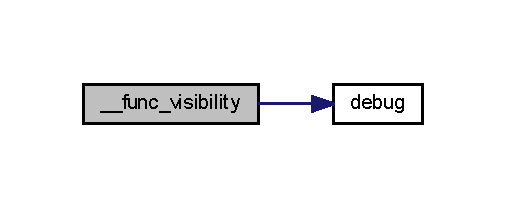
\includegraphics[width=243pt]{_declaring___attributes__of___functions_8h_a6307cb225a3697c3c667e46fb27c3a74_cgraph}
\end{center}
\end{figure}
\mbox{\Hypertarget{_declaring___attributes__of___functions_8h_a1b1e21f7bd1cc25b71a72304b05004cd}\label{_declaring___attributes__of___functions_8h_a1b1e21f7bd1cc25b71a72304b05004cd}} 
\index{Declaring\+\_\+\+Attributes\+\_\+of\+\_\+\+Functions.\+h@{Declaring\+\_\+\+Attributes\+\_\+of\+\_\+\+Functions.\+h}!\+\_\+\+\_\+func\+\_\+warn\+\_\+unused\+\_\+result@{\+\_\+\+\_\+func\+\_\+warn\+\_\+unused\+\_\+result}}
\index{\+\_\+\+\_\+func\+\_\+warn\+\_\+unused\+\_\+result@{\+\_\+\+\_\+func\+\_\+warn\+\_\+unused\+\_\+result}!Declaring\+\_\+\+Attributes\+\_\+of\+\_\+\+Functions.\+h@{Declaring\+\_\+\+Attributes\+\_\+of\+\_\+\+Functions.\+h}}
\subsubsection{\texorpdfstring{\+\_\+\+\_\+func\+\_\+warn\+\_\+unused\+\_\+result()}{\_\_func\_warn\_unused\_result()}}
{\footnotesize\ttfamily int \+\_\+\+\_\+func\+\_\+warn\+\_\+unused\+\_\+result (\begin{DoxyParamCaption}\item[{void}]{ }\end{DoxyParamCaption})}

\mbox{\Hypertarget{_declaring___attributes__of___functions_8h_ab057dfa6daeabaf2388048dc18b5a794}\label{_declaring___attributes__of___functions_8h_ab057dfa6daeabaf2388048dc18b5a794}} 
\index{Declaring\+\_\+\+Attributes\+\_\+of\+\_\+\+Functions.\+h@{Declaring\+\_\+\+Attributes\+\_\+of\+\_\+\+Functions.\+h}!\+\_\+\+\_\+func\+\_\+weakref@{\+\_\+\+\_\+func\+\_\+weakref}}
\index{\+\_\+\+\_\+func\+\_\+weakref@{\+\_\+\+\_\+func\+\_\+weakref}!Declaring\+\_\+\+Attributes\+\_\+of\+\_\+\+Functions.\+h@{Declaring\+\_\+\+Attributes\+\_\+of\+\_\+\+Functions.\+h}}
\subsubsection{\texorpdfstring{\+\_\+\+\_\+func\+\_\+weakref()}{\_\_func\_weakref()}}
{\footnotesize\ttfamily void \+\_\+\+\_\+func\+\_\+weakref (\begin{DoxyParamCaption}\item[{void}]{ }\end{DoxyParamCaption})}

\mbox{\Hypertarget{_declaring___attributes__of___functions_8h_a8f556a5a59e1162e11b05baec39ee3f9}\label{_declaring___attributes__of___functions_8h_a8f556a5a59e1162e11b05baec39ee3f9}} 
\index{Declaring\+\_\+\+Attributes\+\_\+of\+\_\+\+Functions.\+h@{Declaring\+\_\+\+Attributes\+\_\+of\+\_\+\+Functions.\+h}!debug@{debug}}
\index{debug@{debug}!Declaring\+\_\+\+Attributes\+\_\+of\+\_\+\+Functions.\+h@{Declaring\+\_\+\+Attributes\+\_\+of\+\_\+\+Functions.\+h}}
\subsubsection{\texorpdfstring{debug()}{debug()}}
{\footnotesize\ttfamily void void debug (\begin{DoxyParamCaption}\item[{int}]{dlevel,  }\item[{const char $\ast$}]{format,  }\item[{}]{... }\end{DoxyParamCaption})}

\mbox{\Hypertarget{_declaring___attributes__of___functions_8h_ad8bf4027913439e0459739896645d771}\label{_declaring___attributes__of___functions_8h_ad8bf4027913439e0459739896645d771}} 
\index{Declaring\+\_\+\+Attributes\+\_\+of\+\_\+\+Functions.\+h@{Declaring\+\_\+\+Attributes\+\_\+of\+\_\+\+Functions.\+h}!error@{error}}
\index{error@{error}!Declaring\+\_\+\+Attributes\+\_\+of\+\_\+\+Functions.\+h@{Declaring\+\_\+\+Attributes\+\_\+of\+\_\+\+Functions.\+h}}
\subsubsection{\texorpdfstring{error()}{error()}}
{\footnotesize\ttfamily void error (\begin{DoxyParamCaption}\item[{const char $\ast$}]{format,  }\item[{}]{... }\end{DoxyParamCaption})}

\mbox{\Hypertarget{_declaring___attributes__of___functions_8h_ace09e9735ddb34c9cf9e6de2ebb2be49}\label{_declaring___attributes__of___functions_8h_ace09e9735ddb34c9cf9e6de2ebb2be49}} 
\index{Declaring\+\_\+\+Attributes\+\_\+of\+\_\+\+Functions.\+h@{Declaring\+\_\+\+Attributes\+\_\+of\+\_\+\+Functions.\+h}!f\+\_\+nonnull@{f\+\_\+nonnull}}
\index{f\+\_\+nonnull@{f\+\_\+nonnull}!Declaring\+\_\+\+Attributes\+\_\+of\+\_\+\+Functions.\+h@{Declaring\+\_\+\+Attributes\+\_\+of\+\_\+\+Functions.\+h}}
\subsubsection{\texorpdfstring{f\+\_\+nonnull()}{f\_nonnull()}}
{\footnotesize\ttfamily void f\+\_\+nonnull (\begin{DoxyParamCaption}\item[{void $\ast$}]{dest,  }\item[{const void $\ast$}]{src,  }\item[{size\+\_\+t}]{len }\end{DoxyParamCaption})}

\mbox{\Hypertarget{_declaring___attributes__of___functions_8h_a2f9582bef5dfe15aab08367e45e02a3f}\label{_declaring___attributes__of___functions_8h_a2f9582bef5dfe15aab08367e45e02a3f}} 
\index{Declaring\+\_\+\+Attributes\+\_\+of\+\_\+\+Functions.\+h@{Declaring\+\_\+\+Attributes\+\_\+of\+\_\+\+Functions.\+h}!f\+\_\+noreturn@{f\+\_\+noreturn}}
\index{f\+\_\+noreturn@{f\+\_\+noreturn}!Declaring\+\_\+\+Attributes\+\_\+of\+\_\+\+Functions.\+h@{Declaring\+\_\+\+Attributes\+\_\+of\+\_\+\+Functions.\+h}}
\subsubsection{\texorpdfstring{f\+\_\+noreturn()}{f\_noreturn()}}
{\footnotesize\ttfamily void f\+\_\+noreturn (\begin{DoxyParamCaption}\item[{void}]{ }\end{DoxyParamCaption})}



Declaring\+\_\+\+Attributes\+\_\+of\+\_\+\+Functions.\+c 파일의 13 번째 라인에서 정의되었습니다.


\begin{DoxyCode}
16 \{
17     \hyperlink{_declaring___attributes__of___functions_8c_a677a2f44d0dc12217eb3ccbbc623f8ba}{debug}(1, \textcolor{stringliteral}{"%s is called..\(\backslash\)n"}, \_\_func\_\_);
18 \}
\end{DoxyCode}
\mbox{\Hypertarget{_declaring___attributes__of___functions_8h_a1a2fc7e33ab06ba46dc47f7c63c3f60e}\label{_declaring___attributes__of___functions_8h_a1a2fc7e33ab06ba46dc47f7c63c3f60e}} 
\index{Declaring\+\_\+\+Attributes\+\_\+of\+\_\+\+Functions.\+h@{Declaring\+\_\+\+Attributes\+\_\+of\+\_\+\+Functions.\+h}!f\+\_\+visibility@{f\+\_\+visibility}}
\index{f\+\_\+visibility@{f\+\_\+visibility}!Declaring\+\_\+\+Attributes\+\_\+of\+\_\+\+Functions.\+h@{Declaring\+\_\+\+Attributes\+\_\+of\+\_\+\+Functions.\+h}}
\subsubsection{\texorpdfstring{f\+\_\+visibility()}{f\_visibility()}}
{\footnotesize\ttfamily void f\+\_\+visibility (\begin{DoxyParamCaption}\item[{void}]{ }\end{DoxyParamCaption})}



Declaring\+\_\+\+Attributes\+\_\+of\+\_\+\+Functions.\+c 파일의 27 번째 라인에서 정의되었습니다.


\begin{DoxyCode}
31 \{
32     \hyperlink{_declaring___attributes__of___functions_8c_a677a2f44d0dc12217eb3ccbbc623f8ba}{debug}(1, \textcolor{stringliteral}{"%s is called..\(\backslash\)n"}, \_\_func\_\_);
33     \textcolor{keywordflow}{return} 0;
34 \}
\end{DoxyCode}
\mbox{\Hypertarget{_declaring___attributes__of___functions_8h_a53dea1426a2c6d2c6f792cbc78aacc96}\label{_declaring___attributes__of___functions_8h_a53dea1426a2c6d2c6f792cbc78aacc96}} 
\index{Declaring\+\_\+\+Attributes\+\_\+of\+\_\+\+Functions.\+h@{Declaring\+\_\+\+Attributes\+\_\+of\+\_\+\+Functions.\+h}!f\+\_\+warn\+\_\+unused\+\_\+result@{f\+\_\+warn\+\_\+unused\+\_\+result}}
\index{f\+\_\+warn\+\_\+unused\+\_\+result@{f\+\_\+warn\+\_\+unused\+\_\+result}!Declaring\+\_\+\+Attributes\+\_\+of\+\_\+\+Functions.\+h@{Declaring\+\_\+\+Attributes\+\_\+of\+\_\+\+Functions.\+h}}
\subsubsection{\texorpdfstring{f\+\_\+warn\+\_\+unused\+\_\+result()}{f\_warn\_unused\_result()}}
{\footnotesize\ttfamily int f\+\_\+warn\+\_\+unused\+\_\+result (\begin{DoxyParamCaption}\item[{void}]{ }\end{DoxyParamCaption})}



Declaring\+\_\+\+Attributes\+\_\+of\+\_\+\+Functions.\+c 파일의 36 번째 라인에서 정의되었습니다.


\begin{DoxyCode}
39 \{
40     \hyperlink{_declaring___attributes__of___functions_8c_a677a2f44d0dc12217eb3ccbbc623f8ba}{debug}(1, \textcolor{stringliteral}{"%s is called..\(\backslash\)n"}, \_\_func\_\_);
41 \}
\end{DoxyCode}
\mbox{\Hypertarget{_declaring___attributes__of___functions_8h_af729a5eb32486892390961ab15e017f0}\label{_declaring___attributes__of___functions_8h_af729a5eb32486892390961ab15e017f0}} 
\index{Declaring\+\_\+\+Attributes\+\_\+of\+\_\+\+Functions.\+h@{Declaring\+\_\+\+Attributes\+\_\+of\+\_\+\+Functions.\+h}!f\+\_\+weakref@{f\+\_\+weakref}}
\index{f\+\_\+weakref@{f\+\_\+weakref}!Declaring\+\_\+\+Attributes\+\_\+of\+\_\+\+Functions.\+h@{Declaring\+\_\+\+Attributes\+\_\+of\+\_\+\+Functions.\+h}}
\subsubsection{\texorpdfstring{f\+\_\+weakref()}{f\_weakref()}}
{\footnotesize\ttfamily void f\+\_\+weakref (\begin{DoxyParamCaption}\item[{void}]{ }\end{DoxyParamCaption})}



Declaring\+\_\+\+Attributes\+\_\+of\+\_\+\+Functions.\+c 파일의 42 번째 라인에서 정의되었습니다.


\begin{DoxyCode}
45 \{
46     va\_list ap;
47     va\_start (ap, fmt);
48 
49     vfprintf(stderr, fmt, ap);
50     va\_end(ap);   
51 \}
\end{DoxyCode}

\hypertarget{_declaring___attributes__of___functions2_8c}{}\section{src/function/\+Declaring\+\_\+\+Attributes\+\_\+of\+\_\+\+Functions2.c 파일 참조}
\label{_declaring___attributes__of___functions2_8c}\index{src/function/\+Declaring\+\_\+\+Attributes\+\_\+of\+\_\+\+Functions2.\+c@{src/function/\+Declaring\+\_\+\+Attributes\+\_\+of\+\_\+\+Functions2.\+c}}
\subsection*{함수}
\begin{DoxyCompactItemize}
\item 
void \hyperlink{_declaring___attributes__of___functions2_8c_ae6c3c5224cdf31d53c1facae6142e78c}{f\+\_\+external} (void)
\end{DoxyCompactItemize}


\subsection{함수 문서화}
\mbox{\Hypertarget{_declaring___attributes__of___functions2_8c_ae6c3c5224cdf31d53c1facae6142e78c}\label{_declaring___attributes__of___functions2_8c_ae6c3c5224cdf31d53c1facae6142e78c}} 
\index{Declaring\+\_\+\+Attributes\+\_\+of\+\_\+\+Functions2.\+c@{Declaring\+\_\+\+Attributes\+\_\+of\+\_\+\+Functions2.\+c}!f\+\_\+external@{f\+\_\+external}}
\index{f\+\_\+external@{f\+\_\+external}!Declaring\+\_\+\+Attributes\+\_\+of\+\_\+\+Functions2.\+c@{Declaring\+\_\+\+Attributes\+\_\+of\+\_\+\+Functions2.\+c}}
\subsubsection{\texorpdfstring{f\+\_\+external()}{f\_external()}}
{\footnotesize\ttfamily void f\+\_\+external (\begin{DoxyParamCaption}\item[{void}]{ }\end{DoxyParamCaption})}



Declaring\+\_\+\+Attributes\+\_\+of\+\_\+\+Functions2.\+c 파일의 2 번째 라인에서 정의되었습니다.


\begin{DoxyCode}
3 \{
4     f\_hidden();
5 \}
\end{DoxyCode}

\hypertarget{_declaring___attributes__of___functions__main_8c}{}\section{src/function/\+Declaring\+\_\+\+Attributes\+\_\+of\+\_\+\+Functions\+\_\+main.c 파일 참조}
\label{_declaring___attributes__of___functions__main_8c}\index{src/function/\+Declaring\+\_\+\+Attributes\+\_\+of\+\_\+\+Functions\+\_\+main.\+c@{src/function/\+Declaring\+\_\+\+Attributes\+\_\+of\+\_\+\+Functions\+\_\+main.\+c}}
{\ttfamily \#include $<$stdio.\+h$>$}\newline
{\ttfamily \#include $<$linux/types.\+h$>$}\newline
{\ttfamily \#include \char`\"{}Declaring\+\_\+\+Attributes\+\_\+of\+\_\+\+Functions.\+h\char`\"{}}\newline
Declaring\+\_\+\+Attributes\+\_\+of\+\_\+\+Functions\+\_\+main.\+c에 대한 include 의존 그래프
\nopagebreak
\begin{figure}[H]
\begin{center}
\leavevmode
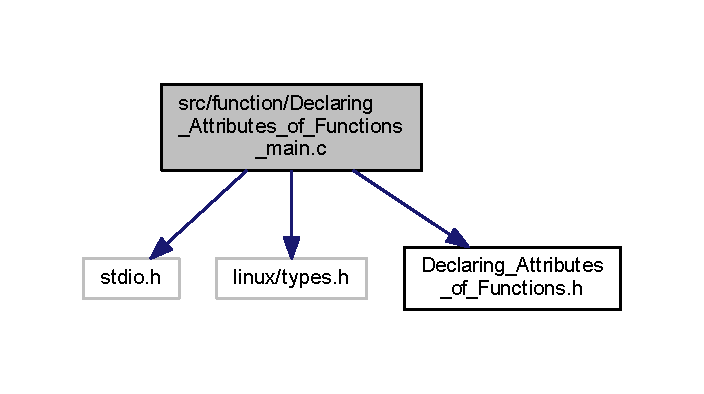
\includegraphics[width=338pt]{_declaring___attributes__of___functions__main_8c__incl}
\end{center}
\end{figure}
\subsection*{함수}
\begin{DoxyCompactItemize}
\item 
static void \hyperlink{_declaring___attributes__of___functions__main_8c_a7a7ebb6dcaca5da0b05940fd85d85854}{stf\+\_\+weakref} (void)
\end{DoxyCompactItemize}
\subsection*{변수}
\begin{DoxyCompactItemize}
\item 
void($\ast$ \hyperlink{_declaring___attributes__of___functions__main_8c_a5eb4882a3de5d038fc36b413cdf7615c}{p\+\_\+func} )(void)
\end{DoxyCompactItemize}


\subsection{함수 문서화}
\mbox{\Hypertarget{_declaring___attributes__of___functions__main_8c_a7a7ebb6dcaca5da0b05940fd85d85854}\label{_declaring___attributes__of___functions__main_8c_a7a7ebb6dcaca5da0b05940fd85d85854}} 
\index{Declaring\+\_\+\+Attributes\+\_\+of\+\_\+\+Functions\+\_\+main.\+c@{Declaring\+\_\+\+Attributes\+\_\+of\+\_\+\+Functions\+\_\+main.\+c}!stf\+\_\+weakref@{stf\+\_\+weakref}}
\index{stf\+\_\+weakref@{stf\+\_\+weakref}!Declaring\+\_\+\+Attributes\+\_\+of\+\_\+\+Functions\+\_\+main.\+c@{Declaring\+\_\+\+Attributes\+\_\+of\+\_\+\+Functions\+\_\+main.\+c}}
\subsubsection{\texorpdfstring{stf\+\_\+weakref()}{stf\_weakref()}}
{\footnotesize\ttfamily static void stf\+\_\+weakref (\begin{DoxyParamCaption}\item[{void}]{ }\end{DoxyParamCaption})\hspace{0.3cm}{\ttfamily [static]}}



Declaring\+\_\+\+Attributes\+\_\+of\+\_\+\+Functions\+\_\+main.\+c 파일의 7 번째 라인에서 정의되었습니다.


\begin{DoxyCode}
10 \{
11     \textcolor{comment}{/* f\_noreturn(); */}
12     \hyperlink{_declaring___attributes__of___functions_8c_ae4dd766abad745c5113303b9ea06c8de}{f\_nonnull}(NULL, NULL, 0);
13     \hyperlink{_declaring___attributes__of___functions__main_8c_a5eb4882a3de5d038fc36b413cdf7615c}{p\_func}();
14     \hyperlink{_declaring___attributes__of___functions_8c_af7e19d11f45bdef39e05946fa24aafd0}{f\_warn\_unused\_result}();
15     \hyperlink{_declaring___attributes__of___functions__main_8c_a7a7ebb6dcaca5da0b05940fd85d85854}{stf\_weakref}();
16 
17     \textcolor{keywordflow}{return} 0;
18 \}
\end{DoxyCode}


\subsection{변수 문서화}
\mbox{\Hypertarget{_declaring___attributes__of___functions__main_8c_a5eb4882a3de5d038fc36b413cdf7615c}\label{_declaring___attributes__of___functions__main_8c_a5eb4882a3de5d038fc36b413cdf7615c}} 
\index{Declaring\+\_\+\+Attributes\+\_\+of\+\_\+\+Functions\+\_\+main.\+c@{Declaring\+\_\+\+Attributes\+\_\+of\+\_\+\+Functions\+\_\+main.\+c}!p\+\_\+func@{p\+\_\+func}}
\index{p\+\_\+func@{p\+\_\+func}!Declaring\+\_\+\+Attributes\+\_\+of\+\_\+\+Functions\+\_\+main.\+c@{Declaring\+\_\+\+Attributes\+\_\+of\+\_\+\+Functions\+\_\+main.\+c}}
\subsubsection{\texorpdfstring{p\+\_\+func}{p\_func}}
{\footnotesize\ttfamily void($\ast$ p\+\_\+func) (void)}


\hypertarget{function_2main_8c}{}\section{src/function/main.c 파일 참조}
\label{function_2main_8c}\index{src/function/main.\+c@{src/function/main.\+c}}
{\ttfamily \#include $<$stdint.\+h$>$}\newline
{\ttfamily \#include $<$stdio.\+h$>$}\newline
{\ttfamily \#include $<$stddef.\+h$>$}\newline
{\ttfamily \#include $<$stdlib.\+h$>$}\newline
{\ttfamily \#include $<$string.\+h$>$}\newline
{\ttfamily \#include $<$stdarg.\+h$>$}\newline
{\ttfamily \#include $<$errno.\+h$>$}\newline
{\ttfamily \#include $<$assert.\+h$>$}\newline
{\ttfamily \#include $<$time.\+h$>$}\newline
main.\+c에 대한 include 의존 그래프
\nopagebreak
\begin{figure}[H]
\begin{center}
\leavevmode
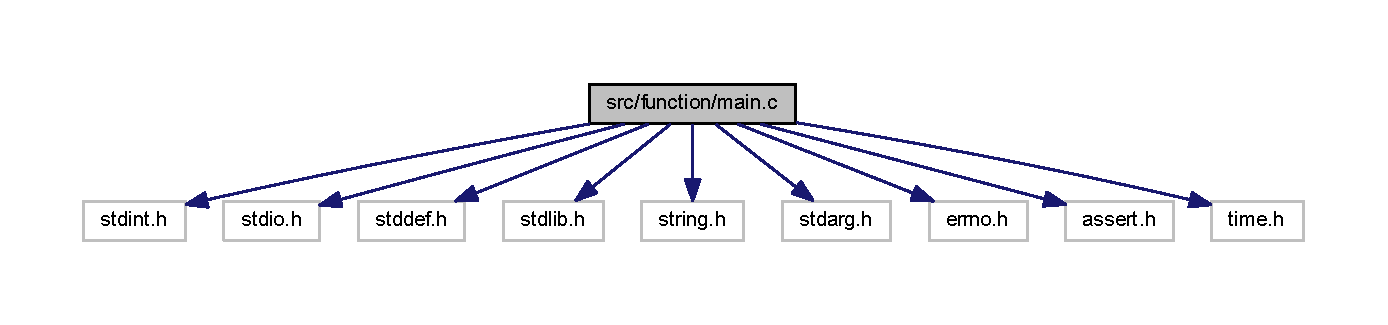
\includegraphics[width=350pt]{function_2main_8c__incl}
\end{center}
\end{figure}
\subsection*{데이터 구조}
\begin{DoxyCompactItemize}
\item 
struct \hyperlink{structinventory}{inventory}
\end{DoxyCompactItemize}
\subsection*{매크로}
\begin{DoxyCompactItemize}
\item 
\#define \hyperlink{function_2main_8c_a7ec751f49d6391028a94f1419374c2fa}{A\+R\+R\+A\+Y\+\_\+\+S\+I\+ZE}~8
\begin{DoxyCompactList}\small\item\em Array size \end{DoxyCompactList}\item 
\#define \hyperlink{function_2main_8c_a6c7cd32e1bac137f05e4a752b4ad10af}{B\+U\+F\+F\+\_\+\+S\+I\+ZE}~256
\begin{DoxyCompactList}\small\item\em Buffer size for character data \end{DoxyCompactList}\end{DoxyCompactItemize}
\subsection*{타입정의}
\begin{DoxyCompactItemize}
\item 
typedef struct \hyperlink{structinventory}{inventory} \hyperlink{function_2main_8c_a8c22703abfe0363a35bcceb330525b98}{I\+N\+V\+E\+N\+T\+O\+RY}
\end{DoxyCompactItemize}
\subsection*{함수}
\begin{DoxyCompactItemize}
\item 
void \hyperlink{function_2main_8c_a9a64d615ba104f0ea5a4227ce30e144f}{operation\+Error} (char $\ast$fmt,...)
\item 
void \hyperlink{function_2main_8c_a89097f1107a1598f7c646fb0f30a5e73}{disp\+Inventory} (\hyperlink{function_2main_8c_a8c22703abfe0363a35bcceb330525b98}{I\+N\+V\+E\+N\+T\+O\+RY} $\ast$ip)
\item 
void \hyperlink{function_2main_8c_a2a7ccc2e362e5149dfc3e349cae6d2a1}{sleep} (int cnt)
\item 
int \hyperlink{function_2main_8c_abf9e6b7e6f15df4b525a2e7705ba3089}{main} (int argc, char const $\ast$argv\mbox{[}$\,$\mbox{]})
\end{DoxyCompactItemize}


\subsection{상세한 설명}
\begin{DoxyAuthor}{작성자}

\end{DoxyAuthor}
\begin{DoxyDate}{날짜}

\end{DoxyDate}
\begin{DoxySeeAlso}{참고}

\end{DoxySeeAlso}


\subsection{매크로 문서화}
\mbox{\Hypertarget{function_2main_8c_a7ec751f49d6391028a94f1419374c2fa}\label{function_2main_8c_a7ec751f49d6391028a94f1419374c2fa}} 
\index{function/main.\+c@{function/main.\+c}!A\+R\+R\+A\+Y\+\_\+\+S\+I\+ZE@{A\+R\+R\+A\+Y\+\_\+\+S\+I\+ZE}}
\index{A\+R\+R\+A\+Y\+\_\+\+S\+I\+ZE@{A\+R\+R\+A\+Y\+\_\+\+S\+I\+ZE}!function/main.\+c@{function/main.\+c}}
\subsubsection{\texorpdfstring{A\+R\+R\+A\+Y\+\_\+\+S\+I\+ZE}{ARRAY\_SIZE}}
{\footnotesize\ttfamily \#define A\+R\+R\+A\+Y\+\_\+\+S\+I\+ZE~8}



Array size 



main.\+c 파일의 22 번째 라인에서 정의되었습니다.

\mbox{\Hypertarget{function_2main_8c_a6c7cd32e1bac137f05e4a752b4ad10af}\label{function_2main_8c_a6c7cd32e1bac137f05e4a752b4ad10af}} 
\index{function/main.\+c@{function/main.\+c}!B\+U\+F\+F\+\_\+\+S\+I\+ZE@{B\+U\+F\+F\+\_\+\+S\+I\+ZE}}
\index{B\+U\+F\+F\+\_\+\+S\+I\+ZE@{B\+U\+F\+F\+\_\+\+S\+I\+ZE}!function/main.\+c@{function/main.\+c}}
\subsubsection{\texorpdfstring{B\+U\+F\+F\+\_\+\+S\+I\+ZE}{BUFF\_SIZE}}
{\footnotesize\ttfamily \#define B\+U\+F\+F\+\_\+\+S\+I\+ZE~256}



Buffer size for character data 



main.\+c 파일의 23 번째 라인에서 정의되었습니다.



\subsection{타입정의 문서화}
\mbox{\Hypertarget{function_2main_8c_a8c22703abfe0363a35bcceb330525b98}\label{function_2main_8c_a8c22703abfe0363a35bcceb330525b98}} 
\index{function/main.\+c@{function/main.\+c}!I\+N\+V\+E\+N\+T\+O\+RY@{I\+N\+V\+E\+N\+T\+O\+RY}}
\index{I\+N\+V\+E\+N\+T\+O\+RY@{I\+N\+V\+E\+N\+T\+O\+RY}!function/main.\+c@{function/main.\+c}}
\subsubsection{\texorpdfstring{I\+N\+V\+E\+N\+T\+O\+RY}{INVENTORY}}
{\footnotesize\ttfamily typedef struct \hyperlink{structinventory}{inventory}  \hyperlink{function_2main_8c_a8c22703abfe0363a35bcceb330525b98}{I\+N\+V\+E\+N\+T\+O\+RY}}

상품 재고 관리용 inventory 구조체 정의 

\subsection{함수 문서화}
\mbox{\Hypertarget{function_2main_8c_a89097f1107a1598f7c646fb0f30a5e73}\label{function_2main_8c_a89097f1107a1598f7c646fb0f30a5e73}} 
\index{function/main.\+c@{function/main.\+c}!disp\+Inventory@{disp\+Inventory}}
\index{disp\+Inventory@{disp\+Inventory}!function/main.\+c@{function/main.\+c}}
\subsubsection{\texorpdfstring{disp\+Inventory()}{dispInventory()}}
{\footnotesize\ttfamily void disp\+Inventory (\begin{DoxyParamCaption}\item[{\hyperlink{function_2main_8c_a8c22703abfe0363a35bcceb330525b98}{I\+N\+V\+E\+N\+T\+O\+RY} $\ast$}]{ip }\end{DoxyParamCaption})}


\begin{DoxyParams}{매개변수}
{\em } & \\
\hline
\end{DoxyParams}


main.\+c 파일의 85 번째 라인에서 정의되었습니다.


\begin{DoxyCode}
85                                   \{
86   printf(\textcolor{stringliteral}{"상품명 : %s\(\backslash\)n"}, ip->\hyperlink{structinventory_a5ac083a645d964373f022d03df4849c8}{name});
87   printf(\textcolor{stringliteral}{"상품번호 : %s\(\backslash\)n"}, ip->\hyperlink{structinventory_a77370bcefb3fe21e5f84e230581a50d7}{number});
88   printf(\textcolor{stringliteral}{"재고 수량 : %d\(\backslash\)n"}, ip->\hyperlink{structinventory_aed48ca0bcd2162fd4fd495873e2631f5}{volume});
89   printf(\textcolor{stringliteral}{"매입 일수 : %d\(\backslash\)n"}, ip->\hyperlink{structinventory_ae0484109745ac918f2b3ed8551b41dcb}{leadtime});
90 \}
\end{DoxyCode}
이 함수를 호출하는 함수들에 대한 그래프입니다.\+:
\nopagebreak
\begin{figure}[H]
\begin{center}
\leavevmode
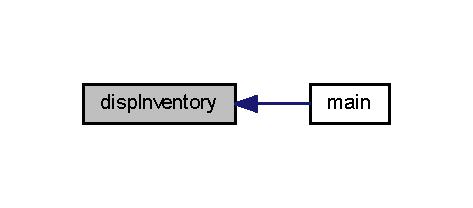
\includegraphics[width=227pt]{function_2main_8c_a89097f1107a1598f7c646fb0f30a5e73_icgraph}
\end{center}
\end{figure}
\mbox{\Hypertarget{function_2main_8c_abf9e6b7e6f15df4b525a2e7705ba3089}\label{function_2main_8c_abf9e6b7e6f15df4b525a2e7705ba3089}} 
\index{function/main.\+c@{function/main.\+c}!main@{main}}
\index{main@{main}!function/main.\+c@{function/main.\+c}}
\subsubsection{\texorpdfstring{main()}{main()}}
{\footnotesize\ttfamily int main (\begin{DoxyParamCaption}\item[{int}]{argc,  }\item[{char const $\ast$}]{argv\mbox{[}$\,$\mbox{]} }\end{DoxyParamCaption})}



main.\+c 파일의 106 번째 라인에서 정의되었습니다.


\begin{DoxyCode}
106                                        \{
107 
108   \textcolor{keywordflow}{return} 0;
109 \}
\end{DoxyCode}
이 함수 내부에서 호출하는 함수들에 대한 그래프입니다.\+:
\nopagebreak
\begin{figure}[H]
\begin{center}
\leavevmode
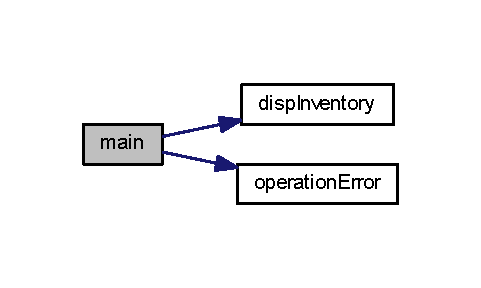
\includegraphics[width=231pt]{function_2main_8c_abf9e6b7e6f15df4b525a2e7705ba3089_cgraph}
\end{center}
\end{figure}
\mbox{\Hypertarget{function_2main_8c_a9a64d615ba104f0ea5a4227ce30e144f}\label{function_2main_8c_a9a64d615ba104f0ea5a4227ce30e144f}} 
\index{function/main.\+c@{function/main.\+c}!operation\+Error@{operation\+Error}}
\index{operation\+Error@{operation\+Error}!function/main.\+c@{function/main.\+c}}
\subsubsection{\texorpdfstring{operation\+Error()}{operationError()}}
{\footnotesize\ttfamily void operation\+Error (\begin{DoxyParamCaption}\item[{char $\ast$}]{fmt,  }\item[{}]{... }\end{DoxyParamCaption})}


\begin{DoxyParams}{매개변수}
{\em } & \\
\hline
\end{DoxyParams}


main.\+c 파일의 64 번째 라인에서 정의되었습니다.


\begin{DoxyCode}
65 \{
66   \textcolor{keywordtype}{char} buff[\hyperlink{function_2main_8c_a6c7cd32e1bac137f05e4a752b4ad10af}{BUFF\_SIZE}] = \{\textcolor{charliteral}{'\(\backslash\)0'}\};
67   va\_list ap;
68 
69   strcpy(buff, \textcolor{stringliteral}{"ERROR: "});
70   va\_start(ap, fmt);
71   vsprintf(buff + strlen(buff), fmt, ap);
72   va\_end(ap);
73 
74   \textcolor{keywordflow}{if} (puts(buff) == EOF) \{
75     printf(\textcolor{stringliteral}{"Failed to write data to stdout!"});
76   \}
77 
78   exit(1);
79 \}
\end{DoxyCode}
이 함수를 호출하는 함수들에 대한 그래프입니다.\+:
\nopagebreak
\begin{figure}[H]
\begin{center}
\leavevmode
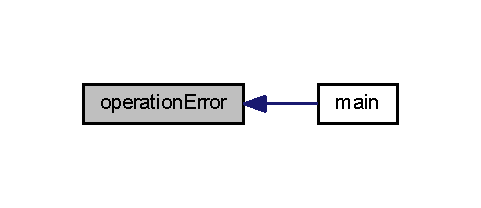
\includegraphics[width=231pt]{function_2main_8c_a9a64d615ba104f0ea5a4227ce30e144f_icgraph}
\end{center}
\end{figure}
\mbox{\Hypertarget{function_2main_8c_a2a7ccc2e362e5149dfc3e349cae6d2a1}\label{function_2main_8c_a2a7ccc2e362e5149dfc3e349cae6d2a1}} 
\index{function/main.\+c@{function/main.\+c}!sleep@{sleep}}
\index{sleep@{sleep}!function/main.\+c@{function/main.\+c}}
\subsubsection{\texorpdfstring{sleep()}{sleep()}}
{\footnotesize\ttfamily void sleep (\begin{DoxyParamCaption}\item[{int}]{cnt }\end{DoxyParamCaption})}


\begin{DoxyParams}{매개변수}
{\em } & \\
\hline
\end{DoxyParams}


main.\+c 파일의 96 번째 라인에서 정의되었습니다.


\begin{DoxyCode}
96                     \{
97   clock\_t t = clock() * (1000 / CLOCKS\_PER\_SEC);
98   clock\_t tterm = t + cnt;
99 
100   \textcolor{keywordflow}{while} (t < tterm) \{
101     t = clock() * (1000 / CLOCKS\_PER\_SEC);
102   \}
103 \}
\end{DoxyCode}

\hypertarget{pointer_2main_8c}{}\section{src/pointer/main.c 파일 참조}
\label{pointer_2main_8c}\index{src/pointer/main.\+c@{src/pointer/main.\+c}}
{\ttfamily \#include $<$stdint.\+h$>$}\newline
{\ttfamily \#include $<$stddef.\+h$>$}\newline
{\ttfamily \#include $<$stdarg.\+h$>$}\newline
{\ttfamily \#include $<$stdio.\+h$>$}\newline
{\ttfamily \#include $<$string.\+h$>$}\newline
{\ttfamily \#include $<$stdlib.\+h$>$}\newline
{\ttfamily \#include \char`\"{}../../inc/ptr.\+h\char`\"{}}\newline
main.\+c에 대한 include 의존 그래프
\nopagebreak
\begin{figure}[H]
\begin{center}
\leavevmode
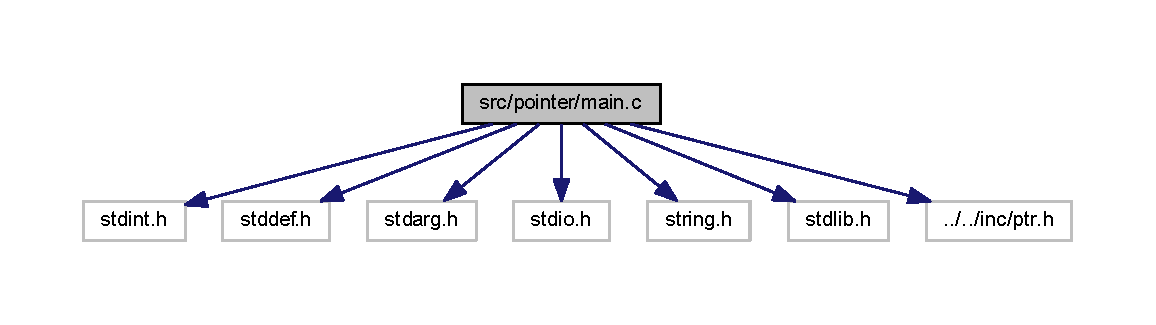
\includegraphics[width=350pt]{pointer_2main_8c__incl}
\end{center}
\end{figure}
\subsection*{매크로}
\begin{DoxyCompactItemize}
\item 
\#define \hyperlink{pointer_2main_8c_a06fc4a42cf3c87aafa67518b95e9d588}{R\+O\+W\+\_\+\+M\+AX}~5
\item 
\#define \hyperlink{pointer_2main_8c_acfbfe944504a5571a1d787b824167ae5}{C\+O\+L\+\_\+\+M\+AX}~10
\end{DoxyCompactItemize}
\subsection*{함수}
\begin{DoxyCompactItemize}
\item 
int \hyperlink{pointer_2main_8c_a64c368cc35a4253d2dfbdfaf19471e8d}{va\+Printf} (char $\ast$fmt,...)
\item 
int \hyperlink{pointer_2main_8c_ac13a0fdb1a48f5ee6712aaa0e830cfda}{main} (int ar\+Tgc, char const $\ast$argv\mbox{[}$\,$\mbox{]})
\end{DoxyCompactItemize}
\subsection*{변수}
\begin{DoxyCompactItemize}
\item 
int $\ast$$\ast$ \hyperlink{pointer_2main_8c_a08d5dd43347ae29fd27e1e66695dbea8}{a} = N\+U\+LL
\end{DoxyCompactItemize}


\subsection{매크로 문서화}
\mbox{\Hypertarget{pointer_2main_8c_acfbfe944504a5571a1d787b824167ae5}\label{pointer_2main_8c_acfbfe944504a5571a1d787b824167ae5}} 
\index{pointer/main.\+c@{pointer/main.\+c}!C\+O\+L\+\_\+\+M\+AX@{C\+O\+L\+\_\+\+M\+AX}}
\index{C\+O\+L\+\_\+\+M\+AX@{C\+O\+L\+\_\+\+M\+AX}!pointer/main.\+c@{pointer/main.\+c}}
\subsubsection{\texorpdfstring{C\+O\+L\+\_\+\+M\+AX}{COL\_MAX}}
{\footnotesize\ttfamily \#define C\+O\+L\+\_\+\+M\+AX~10}



main.\+c 파일의 10 번째 라인에서 정의되었습니다.

\mbox{\Hypertarget{pointer_2main_8c_a06fc4a42cf3c87aafa67518b95e9d588}\label{pointer_2main_8c_a06fc4a42cf3c87aafa67518b95e9d588}} 
\index{pointer/main.\+c@{pointer/main.\+c}!R\+O\+W\+\_\+\+M\+AX@{R\+O\+W\+\_\+\+M\+AX}}
\index{R\+O\+W\+\_\+\+M\+AX@{R\+O\+W\+\_\+\+M\+AX}!pointer/main.\+c@{pointer/main.\+c}}
\subsubsection{\texorpdfstring{R\+O\+W\+\_\+\+M\+AX}{ROW\_MAX}}
{\footnotesize\ttfamily \#define R\+O\+W\+\_\+\+M\+AX~5}



main.\+c 파일의 9 번째 라인에서 정의되었습니다.



\subsection{함수 문서화}
\mbox{\Hypertarget{pointer_2main_8c_ac13a0fdb1a48f5ee6712aaa0e830cfda}\label{pointer_2main_8c_ac13a0fdb1a48f5ee6712aaa0e830cfda}} 
\index{pointer/main.\+c@{pointer/main.\+c}!main@{main}}
\index{main@{main}!pointer/main.\+c@{pointer/main.\+c}}
\subsubsection{\texorpdfstring{main()}{main()}}
{\footnotesize\ttfamily int main (\begin{DoxyParamCaption}\item[{int}]{ar\+Tgc,  }\item[{char const $\ast$}]{argv\mbox{[}$\,$\mbox{]} }\end{DoxyParamCaption})}



main.\+c 파일의 27 번째 라인에서 정의되었습니다.


\begin{DoxyCode}
27                                         \{
28 
29   \textcolor{keywordflow}{return} 0;
30 \}
\end{DoxyCode}
\mbox{\Hypertarget{pointer_2main_8c_a64c368cc35a4253d2dfbdfaf19471e8d}\label{pointer_2main_8c_a64c368cc35a4253d2dfbdfaf19471e8d}} 
\index{pointer/main.\+c@{pointer/main.\+c}!va\+Printf@{va\+Printf}}
\index{va\+Printf@{va\+Printf}!pointer/main.\+c@{pointer/main.\+c}}
\subsubsection{\texorpdfstring{va\+Printf()}{vaPrintf()}}
{\footnotesize\ttfamily int va\+Printf (\begin{DoxyParamCaption}\item[{char $\ast$}]{fmt,  }\item[{}]{... }\end{DoxyParamCaption})}



main.\+c 파일의 14 번째 라인에서 정의되었습니다.


\begin{DoxyCode}
15 \{
16   \textcolor{keywordtype}{char} buf[256] = \{\textcolor{charliteral}{'\(\backslash\)0'},\};
17   va\_list ap;
18 
19   strcpy(buf, \textcolor{stringliteral}{"Error: "});
20   va\_start(ap, fmt);
21   vsprintf(buf + strlen(buf), fmt, ap);
22   va\_end(ap);
23 
24     puts(buf);
25 \}
\end{DoxyCode}


\subsection{변수 문서화}
\mbox{\Hypertarget{pointer_2main_8c_a08d5dd43347ae29fd27e1e66695dbea8}\label{pointer_2main_8c_a08d5dd43347ae29fd27e1e66695dbea8}} 
\index{pointer/main.\+c@{pointer/main.\+c}!a@{a}}
\index{a@{a}!pointer/main.\+c@{pointer/main.\+c}}
\subsubsection{\texorpdfstring{a}{a}}
{\footnotesize\ttfamily int$\ast$$\ast$ a = N\+U\+LL}



main.\+c 파일의 12 번째 라인에서 정의되었습니다.


\hypertarget{structure_8c}{}\section{src/keyword/structure.c 파일 참조}
\label{structure_8c}\index{src/keyword/structure.\+c@{src/keyword/structure.\+c}}
{\ttfamily \#include $<$stdint.\+h$>$}\newline
{\ttfamily \#include $<$stdio.\+h$>$}\newline
{\ttfamily \#include $<$stddef.\+h$>$}\newline
{\ttfamily \#include $<$stdlib.\+h$>$}\newline
{\ttfamily \#include $<$string.\+h$>$}\newline
{\ttfamily \#include $<$stdarg.\+h$>$}\newline
{\ttfamily \#include $<$errno.\+h$>$}\newline
{\ttfamily \#include $<$assert.\+h$>$}\newline
{\ttfamily \#include $<$time.\+h$>$}\newline
structure.\+c에 대한 include 의존 그래프
\nopagebreak
\begin{figure}[H]
\begin{center}
\leavevmode
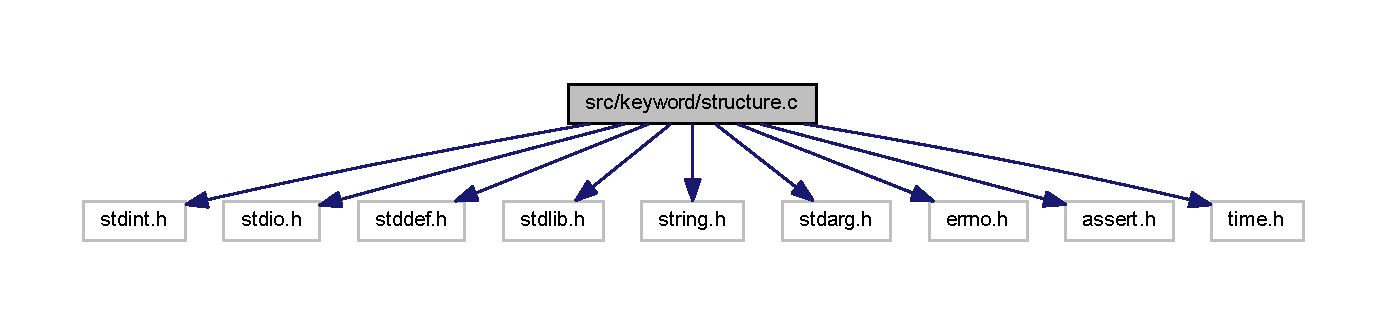
\includegraphics[width=350pt]{structure_8c__incl}
\end{center}
\end{figure}
\subsection*{데이터 구조}
\begin{DoxyCompactItemize}
\item 
struct \hyperlink{struct__struct}{\+\_\+struct}
\end{DoxyCompactItemize}
\subsection*{매크로}
\begin{DoxyCompactItemize}
\item 
\#define \hyperlink{structure_8c_a6c7cd32e1bac137f05e4a752b4ad10af}{B\+U\+F\+F\+\_\+\+S\+I\+ZE}~256
\begin{DoxyCompactList}\small\item\em Buffer size for character data \end{DoxyCompactList}\end{DoxyCompactItemize}
\subsection*{타입정의}
\begin{DoxyCompactItemize}
\item 
typedef struct \hyperlink{struct__struct}{\+\_\+struct} \hyperlink{structure_8c_a6a0147790bea2d2ab884eaf27ce874d1}{S\+T\+R\+U\+CT}
\end{DoxyCompactItemize}
\subsection*{함수}
\begin{DoxyCompactItemize}
\item 
int \hyperlink{structure_8c_abf9e6b7e6f15df4b525a2e7705ba3089}{main} (int argc, char const $\ast$argv\mbox{[}$\,$\mbox{]})
\end{DoxyCompactItemize}


\subsection{상세한 설명}
\begin{DoxyAuthor}{작성자}

\end{DoxyAuthor}
\begin{DoxyDate}{날짜}

\end{DoxyDate}
\begin{DoxySeeAlso}{참고}

\end{DoxySeeAlso}


\subsection{매크로 문서화}
\mbox{\Hypertarget{structure_8c_a6c7cd32e1bac137f05e4a752b4ad10af}\label{structure_8c_a6c7cd32e1bac137f05e4a752b4ad10af}} 
\index{structure.\+c@{structure.\+c}!B\+U\+F\+F\+\_\+\+S\+I\+ZE@{B\+U\+F\+F\+\_\+\+S\+I\+ZE}}
\index{B\+U\+F\+F\+\_\+\+S\+I\+ZE@{B\+U\+F\+F\+\_\+\+S\+I\+ZE}!structure.\+c@{structure.\+c}}
\subsubsection{\texorpdfstring{B\+U\+F\+F\+\_\+\+S\+I\+ZE}{BUFF\_SIZE}}
{\footnotesize\ttfamily \#define B\+U\+F\+F\+\_\+\+S\+I\+ZE~256}



Buffer size for character data 



structure.\+c 파일의 22 번째 라인에서 정의되었습니다.



\subsection{타입정의 문서화}
\mbox{\Hypertarget{structure_8c_a6a0147790bea2d2ab884eaf27ce874d1}\label{structure_8c_a6a0147790bea2d2ab884eaf27ce874d1}} 
\index{structure.\+c@{structure.\+c}!S\+T\+R\+U\+CT@{S\+T\+R\+U\+CT}}
\index{S\+T\+R\+U\+CT@{S\+T\+R\+U\+CT}!structure.\+c@{structure.\+c}}
\subsubsection{\texorpdfstring{S\+T\+R\+U\+CT}{STRUCT}}
{\footnotesize\ttfamily typedef struct \hyperlink{struct__struct}{\+\_\+struct}  \hyperlink{function_2base_8c_a6a0147790bea2d2ab884eaf27ce874d1}{S\+T\+R\+U\+CT}}



\subsection{함수 문서화}
\mbox{\Hypertarget{structure_8c_abf9e6b7e6f15df4b525a2e7705ba3089}\label{structure_8c_abf9e6b7e6f15df4b525a2e7705ba3089}} 
\index{structure.\+c@{structure.\+c}!main@{main}}
\index{main@{main}!structure.\+c@{structure.\+c}}
\subsubsection{\texorpdfstring{main()}{main()}}
{\footnotesize\ttfamily int main (\begin{DoxyParamCaption}\item[{int}]{argc,  }\item[{char const $\ast$}]{argv\mbox{[}$\,$\mbox{]} }\end{DoxyParamCaption})}



structure.\+c 파일의 54 번째 라인에서 정의되었습니다.


\begin{DoxyCode}
54                                        \{
55 
56   \textcolor{keywordflow}{return} 0;
57 \}
\end{DoxyCode}

\hypertarget{abort_8c}{}\section{src/libstd/abort.c 파일 참조}
\label{abort_8c}\index{src/libstd/abort.\+c@{src/libstd/abort.\+c}}
{\ttfamily \#include $<$stdint.\+h$>$}\newline
{\ttfamily \#include $<$stdio.\+h$>$}\newline
{\ttfamily \#include $<$stddef.\+h$>$}\newline
{\ttfamily \#include $<$stdlib.\+h$>$}\newline
{\ttfamily \#include $<$string.\+h$>$}\newline
{\ttfamily \#include $<$stdarg.\+h$>$}\newline
{\ttfamily \#include $<$errno.\+h$>$}\newline
{\ttfamily \#include $<$assert.\+h$>$}\newline
{\ttfamily \#include $<$time.\+h$>$}\newline
abort.\+c에 대한 include 의존 그래프
\nopagebreak
\begin{figure}[H]
\begin{center}
\leavevmode
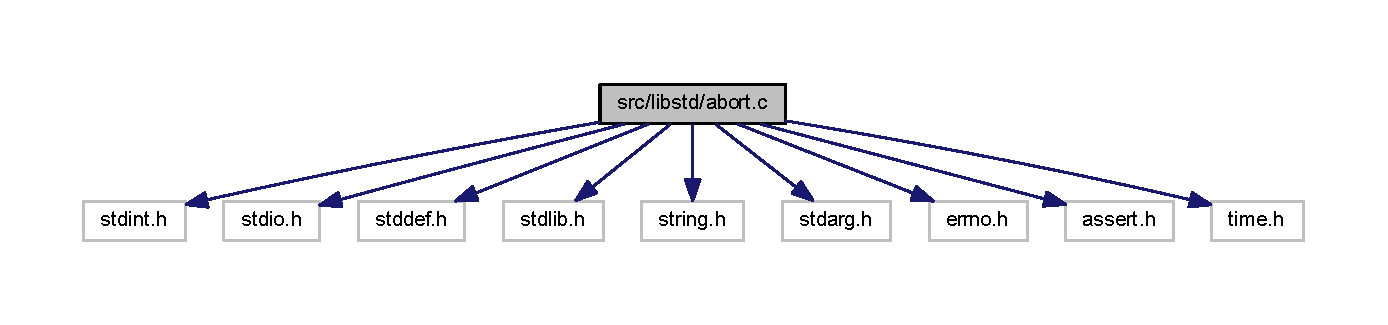
\includegraphics[width=350pt]{abort_8c__incl}
\end{center}
\end{figure}
\subsection*{데이터 구조}
\begin{DoxyCompactItemize}
\item 
struct \hyperlink{struct__struct}{\+\_\+struct}
\end{DoxyCompactItemize}
\subsection*{매크로}
\begin{DoxyCompactItemize}
\item 
\#define \hyperlink{abort_8c_a6c7cd32e1bac137f05e4a752b4ad10af}{B\+U\+F\+F\+\_\+\+S\+I\+ZE}~256
\begin{DoxyCompactList}\small\item\em Buffer size for character data \end{DoxyCompactList}\end{DoxyCompactItemize}
\subsection*{타입정의}
\begin{DoxyCompactItemize}
\item 
typedef struct \hyperlink{struct__struct}{\+\_\+struct} \hyperlink{abort_8c_a6a0147790bea2d2ab884eaf27ce874d1}{S\+T\+R\+U\+CT}
\end{DoxyCompactItemize}
\subsection*{함수}
\begin{DoxyCompactItemize}
\item 
void \hyperlink{abort_8c_ad7451a3c0c566d03a5ac5831e02b0b36}{my\+Abort} (char $\ast$err)
\end{DoxyCompactItemize}


\subsection{상세한 설명}
\begin{DoxyAuthor}{작성자}

\end{DoxyAuthor}
\begin{DoxyDate}{날짜}

\end{DoxyDate}
\begin{DoxySeeAlso}{참고}

\end{DoxySeeAlso}


\subsection{매크로 문서화}
\mbox{\Hypertarget{abort_8c_a6c7cd32e1bac137f05e4a752b4ad10af}\label{abort_8c_a6c7cd32e1bac137f05e4a752b4ad10af}} 
\index{abort.\+c@{abort.\+c}!B\+U\+F\+F\+\_\+\+S\+I\+ZE@{B\+U\+F\+F\+\_\+\+S\+I\+ZE}}
\index{B\+U\+F\+F\+\_\+\+S\+I\+ZE@{B\+U\+F\+F\+\_\+\+S\+I\+ZE}!abort.\+c@{abort.\+c}}
\subsubsection{\texorpdfstring{B\+U\+F\+F\+\_\+\+S\+I\+ZE}{BUFF\_SIZE}}
{\footnotesize\ttfamily \#define B\+U\+F\+F\+\_\+\+S\+I\+ZE~256}



Buffer size for character data 



abort.\+c 파일의 22 번째 라인에서 정의되었습니다.



\subsection{타입정의 문서화}
\mbox{\Hypertarget{abort_8c_a6a0147790bea2d2ab884eaf27ce874d1}\label{abort_8c_a6a0147790bea2d2ab884eaf27ce874d1}} 
\index{abort.\+c@{abort.\+c}!S\+T\+R\+U\+CT@{S\+T\+R\+U\+CT}}
\index{S\+T\+R\+U\+CT@{S\+T\+R\+U\+CT}!abort.\+c@{abort.\+c}}
\subsubsection{\texorpdfstring{S\+T\+R\+U\+CT}{STRUCT}}
{\footnotesize\ttfamily typedef struct \hyperlink{struct__struct}{\+\_\+struct}  \hyperlink{function_2base_8c_a6a0147790bea2d2ab884eaf27ce874d1}{S\+T\+R\+U\+CT}}



\subsection{함수 문서화}
\mbox{\Hypertarget{abort_8c_ad7451a3c0c566d03a5ac5831e02b0b36}\label{abort_8c_ad7451a3c0c566d03a5ac5831e02b0b36}} 
\index{abort.\+c@{abort.\+c}!my\+Abort@{my\+Abort}}
\index{my\+Abort@{my\+Abort}!abort.\+c@{abort.\+c}}
\subsubsection{\texorpdfstring{my\+Abort()}{myAbort()}}
{\footnotesize\ttfamily void my\+Abort (\begin{DoxyParamCaption}\item[{char $\ast$}]{err }\end{DoxyParamCaption})}


\begin{DoxyParams}{매개변수}
{\em } & \\
\hline
\end{DoxyParams}


abort.\+c 파일의 60 번째 라인에서 정의되었습니다.


\begin{DoxyCode}
61 \{
62   \textcolor{keywordtype}{char} buff[256] = \textcolor{stringliteral}{"[ABORT]: "};
63   strncat(buff, err, strlen(err));
64   fprintf(stderr, buff, stderr);
65 \}
\end{DoxyCode}

\hypertarget{clock_8c}{}\section{src/libstd/clock.c 파일 참조}
\label{clock_8c}\index{src/libstd/clock.\+c@{src/libstd/clock.\+c}}
{\ttfamily \#include $<$stdint.\+h$>$}\newline
{\ttfamily \#include $<$stdio.\+h$>$}\newline
{\ttfamily \#include $<$stddef.\+h$>$}\newline
{\ttfamily \#include $<$stdlib.\+h$>$}\newline
{\ttfamily \#include $<$string.\+h$>$}\newline
{\ttfamily \#include $<$stdarg.\+h$>$}\newline
{\ttfamily \#include $<$errno.\+h$>$}\newline
{\ttfamily \#include $<$assert.\+h$>$}\newline
{\ttfamily \#include $<$time.\+h$>$}\newline
clock.\+c에 대한 include 의존 그래프
\nopagebreak
\begin{figure}[H]
\begin{center}
\leavevmode
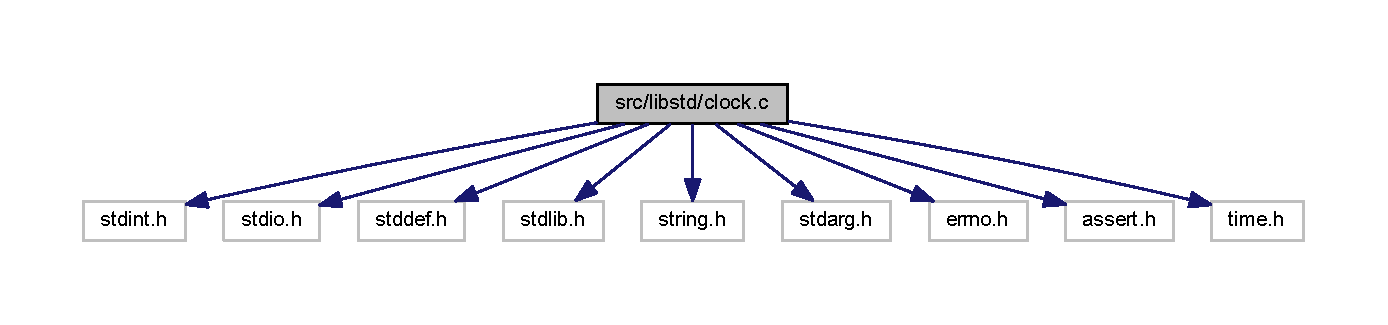
\includegraphics[width=350pt]{clock_8c__incl}
\end{center}
\end{figure}
\subsection*{데이터 구조}
\begin{DoxyCompactItemize}
\item 
struct \hyperlink{structdata__st}{data\+\_\+st}
\end{DoxyCompactItemize}
\subsection*{매크로}
\begin{DoxyCompactItemize}
\item 
\#define \hyperlink{clock_8c_a6c7cd32e1bac137f05e4a752b4ad10af}{B\+U\+F\+F\+\_\+\+S\+I\+ZE}~256
\begin{DoxyCompactList}\small\item\em Buffer size for character data \end{DoxyCompactList}\end{DoxyCompactItemize}
\subsection*{타입정의}
\begin{DoxyCompactItemize}
\item 
typedef struct \hyperlink{structdata__st}{data\+\_\+st} \hyperlink{clock_8c_a8138ab8159c2c3452934cd3f99ceb7a1}{D\+A\+TA}
\end{DoxyCompactItemize}
\subsection*{함수}
\begin{DoxyCompactItemize}
\item 
void \hyperlink{clock_8c_a56b55a3cbf29684da27ef77956e941d3}{my\+Memcpy} (void $\ast$dst, void $\ast$src, unsigned int size)
\end{DoxyCompactItemize}


\subsection{상세한 설명}
\begin{DoxyAuthor}{작성자}

\end{DoxyAuthor}
\begin{DoxyDate}{날짜}

\end{DoxyDate}
\begin{DoxySeeAlso}{참고}

\end{DoxySeeAlso}


\subsection{매크로 문서화}
\mbox{\Hypertarget{clock_8c_a6c7cd32e1bac137f05e4a752b4ad10af}\label{clock_8c_a6c7cd32e1bac137f05e4a752b4ad10af}} 
\index{clock.\+c@{clock.\+c}!B\+U\+F\+F\+\_\+\+S\+I\+ZE@{B\+U\+F\+F\+\_\+\+S\+I\+ZE}}
\index{B\+U\+F\+F\+\_\+\+S\+I\+ZE@{B\+U\+F\+F\+\_\+\+S\+I\+ZE}!clock.\+c@{clock.\+c}}
\subsubsection{\texorpdfstring{B\+U\+F\+F\+\_\+\+S\+I\+ZE}{BUFF\_SIZE}}
{\footnotesize\ttfamily \#define B\+U\+F\+F\+\_\+\+S\+I\+ZE~256}



Buffer size for character data 



clock.\+c 파일의 22 번째 라인에서 정의되었습니다.



\subsection{타입정의 문서화}
\mbox{\Hypertarget{clock_8c_a8138ab8159c2c3452934cd3f99ceb7a1}\label{clock_8c_a8138ab8159c2c3452934cd3f99ceb7a1}} 
\index{clock.\+c@{clock.\+c}!D\+A\+TA@{D\+A\+TA}}
\index{D\+A\+TA@{D\+A\+TA}!clock.\+c@{clock.\+c}}
\subsubsection{\texorpdfstring{D\+A\+TA}{DATA}}
{\footnotesize\ttfamily typedef struct \hyperlink{structdata__st}{data\+\_\+st}  \hyperlink{clock_8c_a8138ab8159c2c3452934cd3f99ceb7a1}{D\+A\+TA}}



\subsection{함수 문서화}
\mbox{\Hypertarget{clock_8c_a56b55a3cbf29684da27ef77956e941d3}\label{clock_8c_a56b55a3cbf29684da27ef77956e941d3}} 
\index{clock.\+c@{clock.\+c}!my\+Memcpy@{my\+Memcpy}}
\index{my\+Memcpy@{my\+Memcpy}!clock.\+c@{clock.\+c}}
\subsubsection{\texorpdfstring{my\+Memcpy()}{myMemcpy()}}
{\footnotesize\ttfamily void my\+Memcpy (\begin{DoxyParamCaption}\item[{void $\ast$}]{dst,  }\item[{void $\ast$}]{src,  }\item[{unsigned int}]{size }\end{DoxyParamCaption})}


\begin{DoxyParams}{매개변수}
{\em } & \\
\hline
\end{DoxyParams}


clock.\+c 파일의 62 번째 라인에서 정의되었습니다.


\begin{DoxyCode}
63  \{
64    \textcolor{keywordtype}{char} *s = src;
65    \textcolor{keywordtype}{char} *d = dst;
66    \textcolor{keywordtype}{size\_t} pad = size % \textcolor{keyword}{sizeof}(int);
67 
68    \textcolor{keywordflow}{for} (\textcolor{keywordtype}{size\_t} i = 0; i < size / \textcolor{keyword}{sizeof}(int); i++) \{
69      *(\textcolor{keywordtype}{int} *)d = *(\textcolor{keywordtype}{int} *)s;
70      s += 4;
71      d += 4;
72    \}
73 
74    \textcolor{keywordflow}{for} (\textcolor{keywordtype}{size\_t} i = 0; i < pad; i++) \{
75      *d = *s;
76      d++;
77      s++;
78    \}
79  \}
\end{DoxyCode}

\hypertarget{common_8h}{}\section{src/libstd/common.h 파일 참조}
\label{common_8h}\index{src/libstd/common.\+h@{src/libstd/common.\+h}}
{\ttfamily \#include $<$stdio.\+h$>$}\newline
common.\+h에 대한 include 의존 그래프
\nopagebreak
\begin{figure}[H]
\begin{center}
\leavevmode
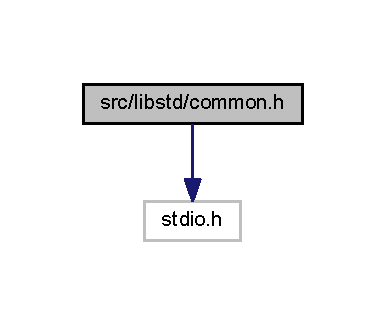
\includegraphics[width=185pt]{common_8h__incl}
\end{center}
\end{figure}

\hypertarget{ptr_8c}{}\section{src/pointer/ptr.c 파일 참조}
\label{ptr_8c}\index{src/pointer/ptr.\+c@{src/pointer/ptr.\+c}}
{\ttfamily \#include $<$stdio.\+h$>$}\newline
{\ttfamily \#include $<$stdlib.\+h$>$}\newline
ptr.\+c에 대한 include 의존 그래프
\nopagebreak
\begin{figure}[H]
\begin{center}
\leavevmode
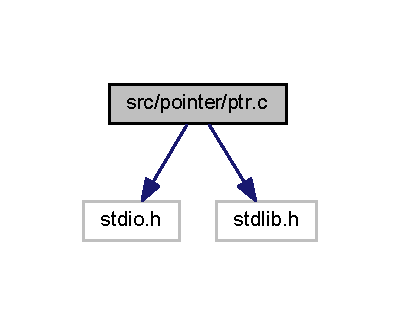
\includegraphics[width=192pt]{ptr_8c__incl}
\end{center}
\end{figure}
\subsection*{매크로}
\begin{DoxyCompactItemize}
\item 
\#define \hyperlink{ptr_8c_a6423a880df59733d2d9b509c7718d3a9}{S\+T\+A\+C\+K\+\_\+\+S\+I\+ZE}~10
\end{DoxyCompactItemize}
\subsection*{타입정의}
\begin{DoxyCompactItemize}
\item 
typedef int \hyperlink{ptr_8c_abdc31db446e3fd2b8884acf9d1132d69}{stack\+\_\+t}
\end{DoxyCompactItemize}
\subsection*{함수}
\begin{DoxyCompactItemize}
\item 
void \hyperlink{ptr_8c_a9235f768e511383f117f41ab92d601f6}{push} (int data)
\item 
int \hyperlink{ptr_8c_a4c5807670c67d62abe111c66c053bd7e}{pop} (void)
\end{DoxyCompactItemize}
\subsection*{변수}
\begin{DoxyCompactItemize}
\item 
\hyperlink{ptr_8c_abdc31db446e3fd2b8884acf9d1132d69}{stack\+\_\+t} \hyperlink{ptr_8c_a460d05636a1abaa5f0f1b51ac0277449}{stack} \mbox{[}\hyperlink{ptr_8c_a6423a880df59733d2d9b509c7718d3a9}{S\+T\+A\+C\+K\+\_\+\+S\+I\+ZE}\mbox{]}
\item 
unsigned int \hyperlink{ptr_8c_a3fdd42ea34070a54e696b3adc28c4be3}{top}
\end{DoxyCompactItemize}


\subsection{매크로 문서화}
\mbox{\Hypertarget{ptr_8c_a6423a880df59733d2d9b509c7718d3a9}\label{ptr_8c_a6423a880df59733d2d9b509c7718d3a9}} 
\index{ptr.\+c@{ptr.\+c}!S\+T\+A\+C\+K\+\_\+\+S\+I\+ZE@{S\+T\+A\+C\+K\+\_\+\+S\+I\+ZE}}
\index{S\+T\+A\+C\+K\+\_\+\+S\+I\+ZE@{S\+T\+A\+C\+K\+\_\+\+S\+I\+ZE}!ptr.\+c@{ptr.\+c}}
\subsubsection{\texorpdfstring{S\+T\+A\+C\+K\+\_\+\+S\+I\+ZE}{STACK\_SIZE}}
{\footnotesize\ttfamily \#define S\+T\+A\+C\+K\+\_\+\+S\+I\+ZE~10}



ptr.\+c 파일의 4 번째 라인에서 정의되었습니다.



\subsection{타입정의 문서화}
\mbox{\Hypertarget{ptr_8c_abdc31db446e3fd2b8884acf9d1132d69}\label{ptr_8c_abdc31db446e3fd2b8884acf9d1132d69}} 
\index{ptr.\+c@{ptr.\+c}!stack\+\_\+t@{stack\+\_\+t}}
\index{stack\+\_\+t@{stack\+\_\+t}!ptr.\+c@{ptr.\+c}}
\subsubsection{\texorpdfstring{stack\+\_\+t}{stack\_t}}
{\footnotesize\ttfamily typedef int \hyperlink{ptr_8c_abdc31db446e3fd2b8884acf9d1132d69}{stack\+\_\+t}}



ptr.\+c 파일의 5 번째 라인에서 정의되었습니다.



\subsection{함수 문서화}
\mbox{\Hypertarget{ptr_8c_a4c5807670c67d62abe111c66c053bd7e}\label{ptr_8c_a4c5807670c67d62abe111c66c053bd7e}} 
\index{ptr.\+c@{ptr.\+c}!pop@{pop}}
\index{pop@{pop}!ptr.\+c@{ptr.\+c}}
\subsubsection{\texorpdfstring{pop()}{pop()}}
{\footnotesize\ttfamily int pop (\begin{DoxyParamCaption}\item[{void}]{ }\end{DoxyParamCaption})}



ptr.\+c 파일의 16 번째 라인에서 정의되었습니다.


\begin{DoxyCode}
17 \{
18   \textcolor{keywordflow}{if} (\hyperlink{ptr_8c_a3fdd42ea34070a54e696b3adc28c4be3}{top} == 0)
19     exit(EXIT\_FAILURE);
20 
21   \textcolor{keywordflow}{return} \hyperlink{ptr_8c_a460d05636a1abaa5f0f1b51ac0277449}{stack}[--\hyperlink{ptr_8c_a3fdd42ea34070a54e696b3adc28c4be3}{top}];
22 \}
\end{DoxyCode}
\mbox{\Hypertarget{ptr_8c_a9235f768e511383f117f41ab92d601f6}\label{ptr_8c_a9235f768e511383f117f41ab92d601f6}} 
\index{ptr.\+c@{ptr.\+c}!push@{push}}
\index{push@{push}!ptr.\+c@{ptr.\+c}}
\subsubsection{\texorpdfstring{push()}{push()}}
{\footnotesize\ttfamily void push (\begin{DoxyParamCaption}\item[{int}]{data }\end{DoxyParamCaption})}



ptr.\+c 파일의 9 번째 라인에서 정의되었습니다.


\begin{DoxyCode}
9                     \{
10   \textcolor{keywordflow}{if} (\hyperlink{ptr_8c_a3fdd42ea34070a54e696b3adc28c4be3}{top} >= \hyperlink{ptr_8c_a6423a880df59733d2d9b509c7718d3a9}{STACK\_SIZE})
11     exit(EXIT\_FAILURE);
12 
13   \hyperlink{ptr_8c_a460d05636a1abaa5f0f1b51ac0277449}{stack}[++\hyperlink{ptr_8c_a3fdd42ea34070a54e696b3adc28c4be3}{top}] = data;
14 \}
\end{DoxyCode}


\subsection{변수 문서화}
\mbox{\Hypertarget{ptr_8c_a460d05636a1abaa5f0f1b51ac0277449}\label{ptr_8c_a460d05636a1abaa5f0f1b51ac0277449}} 
\index{ptr.\+c@{ptr.\+c}!stack@{stack}}
\index{stack@{stack}!ptr.\+c@{ptr.\+c}}
\subsubsection{\texorpdfstring{stack}{stack}}
{\footnotesize\ttfamily \hyperlink{ptr_8c_abdc31db446e3fd2b8884acf9d1132d69}{stack\+\_\+t} stack\mbox{[}\hyperlink{ptr_8c_a6423a880df59733d2d9b509c7718d3a9}{S\+T\+A\+C\+K\+\_\+\+S\+I\+ZE}\mbox{]}}



ptr.\+c 파일의 6 번째 라인에서 정의되었습니다.

\mbox{\Hypertarget{ptr_8c_a3fdd42ea34070a54e696b3adc28c4be3}\label{ptr_8c_a3fdd42ea34070a54e696b3adc28c4be3}} 
\index{ptr.\+c@{ptr.\+c}!top@{top}}
\index{top@{top}!ptr.\+c@{ptr.\+c}}
\subsubsection{\texorpdfstring{top}{top}}
{\footnotesize\ttfamily unsigned int top}



ptr.\+c 파일의 7 번째 라인에서 정의되었습니다.


\hypertarget{ptr_8h}{}\section{src/pointer/ptr.h 파일 참조}
\label{ptr_8h}\index{src/pointer/ptr.\+h@{src/pointer/ptr.\+h}}

%--- End generated contents ---

% Index
\backmatter
\newpage
\phantomsection
\clearemptydoublepage
\addcontentsline{toc}{chapter}{색인}
\printindex

\end{document}
